\section{Hardware Components and Constructions}
\subsection{Lightweight Mirror Prototype Construction}
The multifocal ellipsoidal mirror is the most critical component of the detector. A special comprehensive R$\&$D was conducted for the purpose of addressing all the key requirements and to find possible solutions. This R$\&$D was to test and verify the entire possible technological chain of building mirror prototypes on a 1:2 scale. All core parameters of the detector have been checked and/or derived from results of MC simulations. \\
\indent Because there is no mirror support structure no additional material is introduced  within working acceptance, i.e. in front of drift chambers. Therefore the major requirement we needed to satisfy was to build a lightweight and self-supporting combined multifocal mirror consisting of many ellipsoidal mirror facets properly glued together all along their edges. This led to several problems to solve. \\
\indent One of them was to define contact surfaces of adjacent mirror facets that would allow final assembly to be completed without any shape adjustments and leaving no gaps between them. An analytic solution of a system of two equations of the second order that describe two intersecting ellipsoidal surfaces leads to an equation of the fourth order in general form. The solutions for any two intersecting ellipsoidal mirrors of different parameters have been used directly in the design: the line along which two ellipsoidal surfaces intersect is “a flat line of second order”, i.e. that which entirely belongs to one particular well defined plane. This plane coincides with the edge of each of two adjacent facets that had to be glued together.  
\\
\indent One of the R$\&$D goals was to test this possible solution by building three scaled prototype ellipsoidal facets forming a portion of the combined mirror. Complete set of tooling necessary for the thermal shaping of the front and back films, manufacturing of ellipsoidal substrates, assembly of facets and for final trimming have been successfully used. Some parts for tests are shown in Fig. \ref{fig:Proto_4parts}.

\begin{figure}[h]
    \centering
    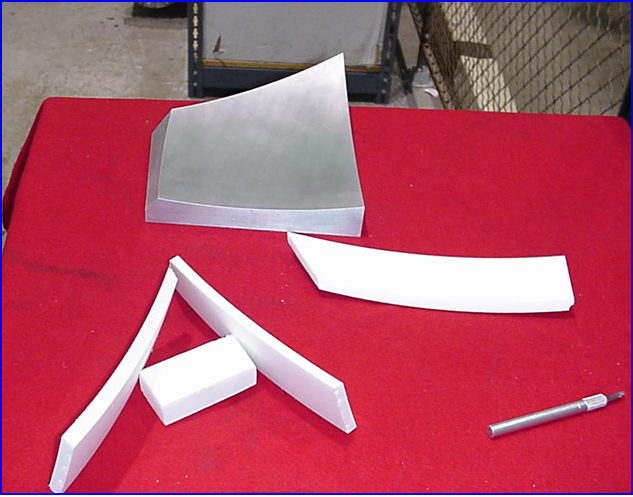
\includegraphics[width=1.0\linewidth]{images/Proto_4parts.png}
    \caption{Three prototype ellipsoidal mirror facets and the spherical master table}
    \label{fig:Proto_4parts}
\end{figure}

Three prototype facets (no reflective coatings on the substrates) were put together touching each other exactly as designed on the spherical working surface of the assembly table. The back of each facet was of same spherical shape. No adjustments were needed at all. We intentionally did not glue them together because the facets have been left under their own weight on the master table of spherical working surface for several months, (see Fig.\ref{fig:Prototype}). We checked for any possible changes in shape and/or in quality.

\begin{figure}[h]
    \centering
    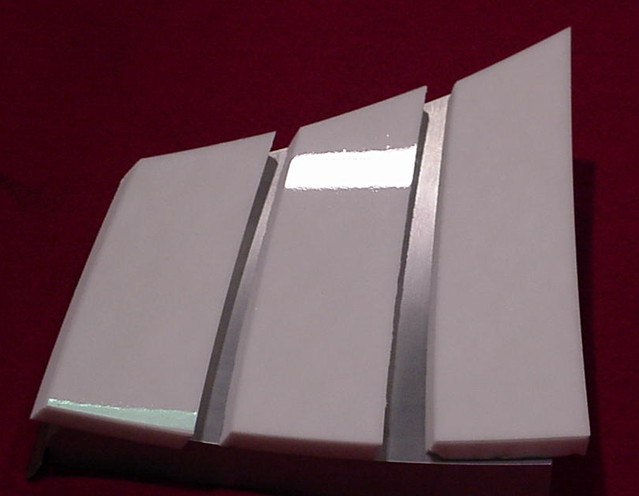
\includegraphics[width=1.0\linewidth]{images/Prototype.png}
    \caption{Three prototype ellipsoidal mirror facets on the spherical master table. They were placed so that they would not touch each other. This was in order to leave them free and to check their shape stability.}
    \label{fig:Prototype}
\end{figure}
We checked for any possible changes in shape and/or for quality of fitting. We have learned the following:

\begin{itemize}
    \item Each substrate must have a sandwiched structure
    \item The thickness of the substrate material has to be between 3/8" and 3/4"
    \item Can use the substrate material ROHACELL polymethacrylimide foam with a density up to 150 mg/cm$^2$
    \item Trimming technology has to be improved to provide increased precision of the mechanical processing and final assembly
    \item In all gluing operations use ether non-shrinking glues or develop a special technique to avoid post-polymerization effects
    \item Acrylic films of optical quality have to be used for the face and back surfaces of the mirrors
    \item It is critical that there is structural stability of the of the set that is being assembled from several mirror facets during gluing process, which includes the complete polymerization time
    \end{itemize}

\indent Obtained results were useful in building the real multifocal mirror. On the Fig.\ref{fig:facet} is shown one of the ellipsoidal facets being prepared for the combined mirror assembly.

\begin{figure}[h]
    \centering
    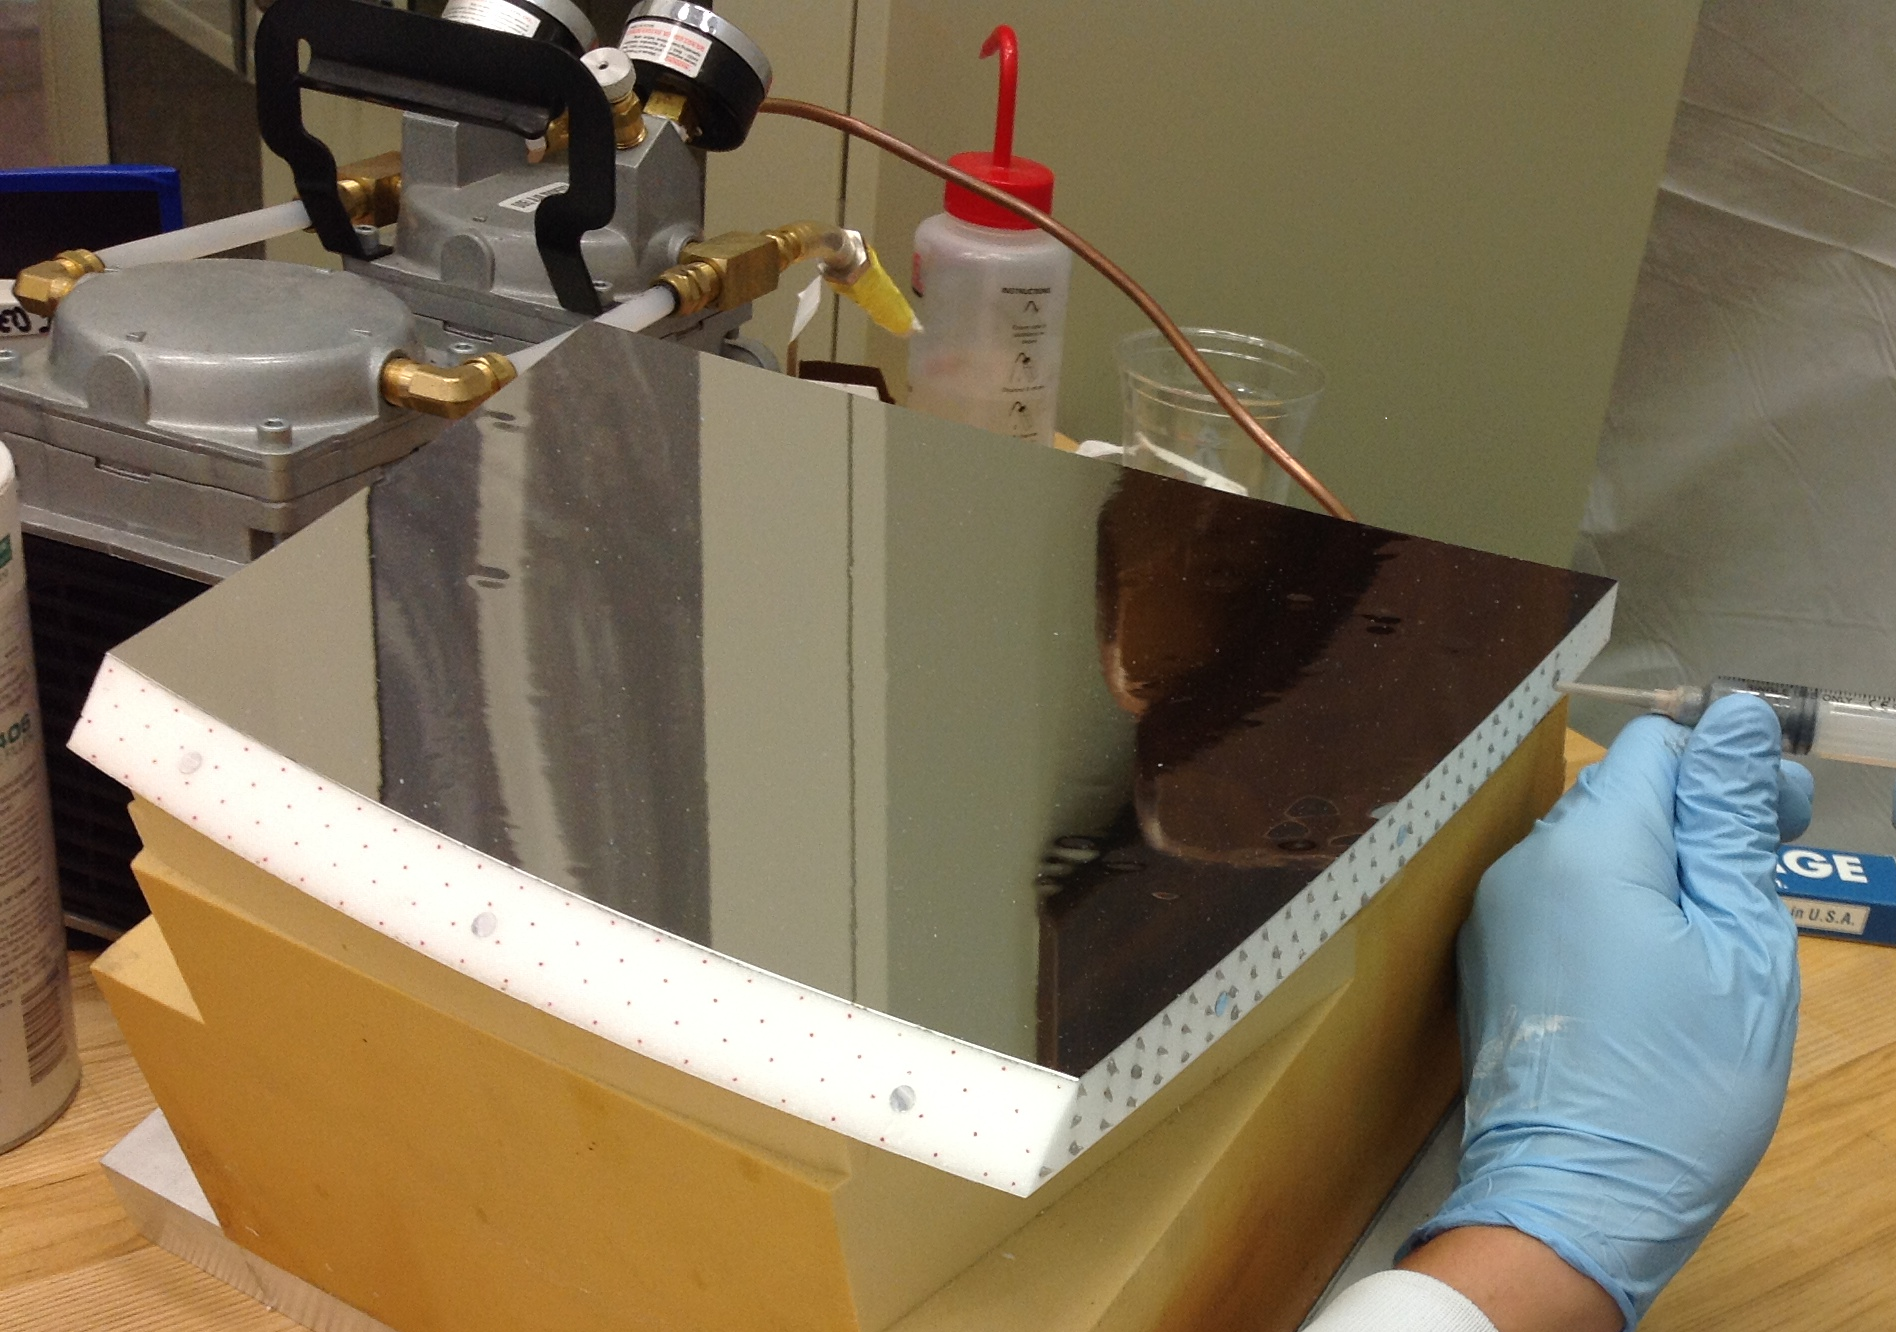
\includegraphics[width=1.0\linewidth]{images/Picture2.png}
    \caption{Ellipsoidal mirror facet has all four flat contact surfaces for gluing}
    \label{fig:facet}
\end{figure}

\indent Final assembly of a 1/12 portion consisting of five ellipsoidal coated mirror facets or one half-sector is illustrated in the Fig.\ref{fig:one_sector}.

\begin{figure}[h]
    \centering
    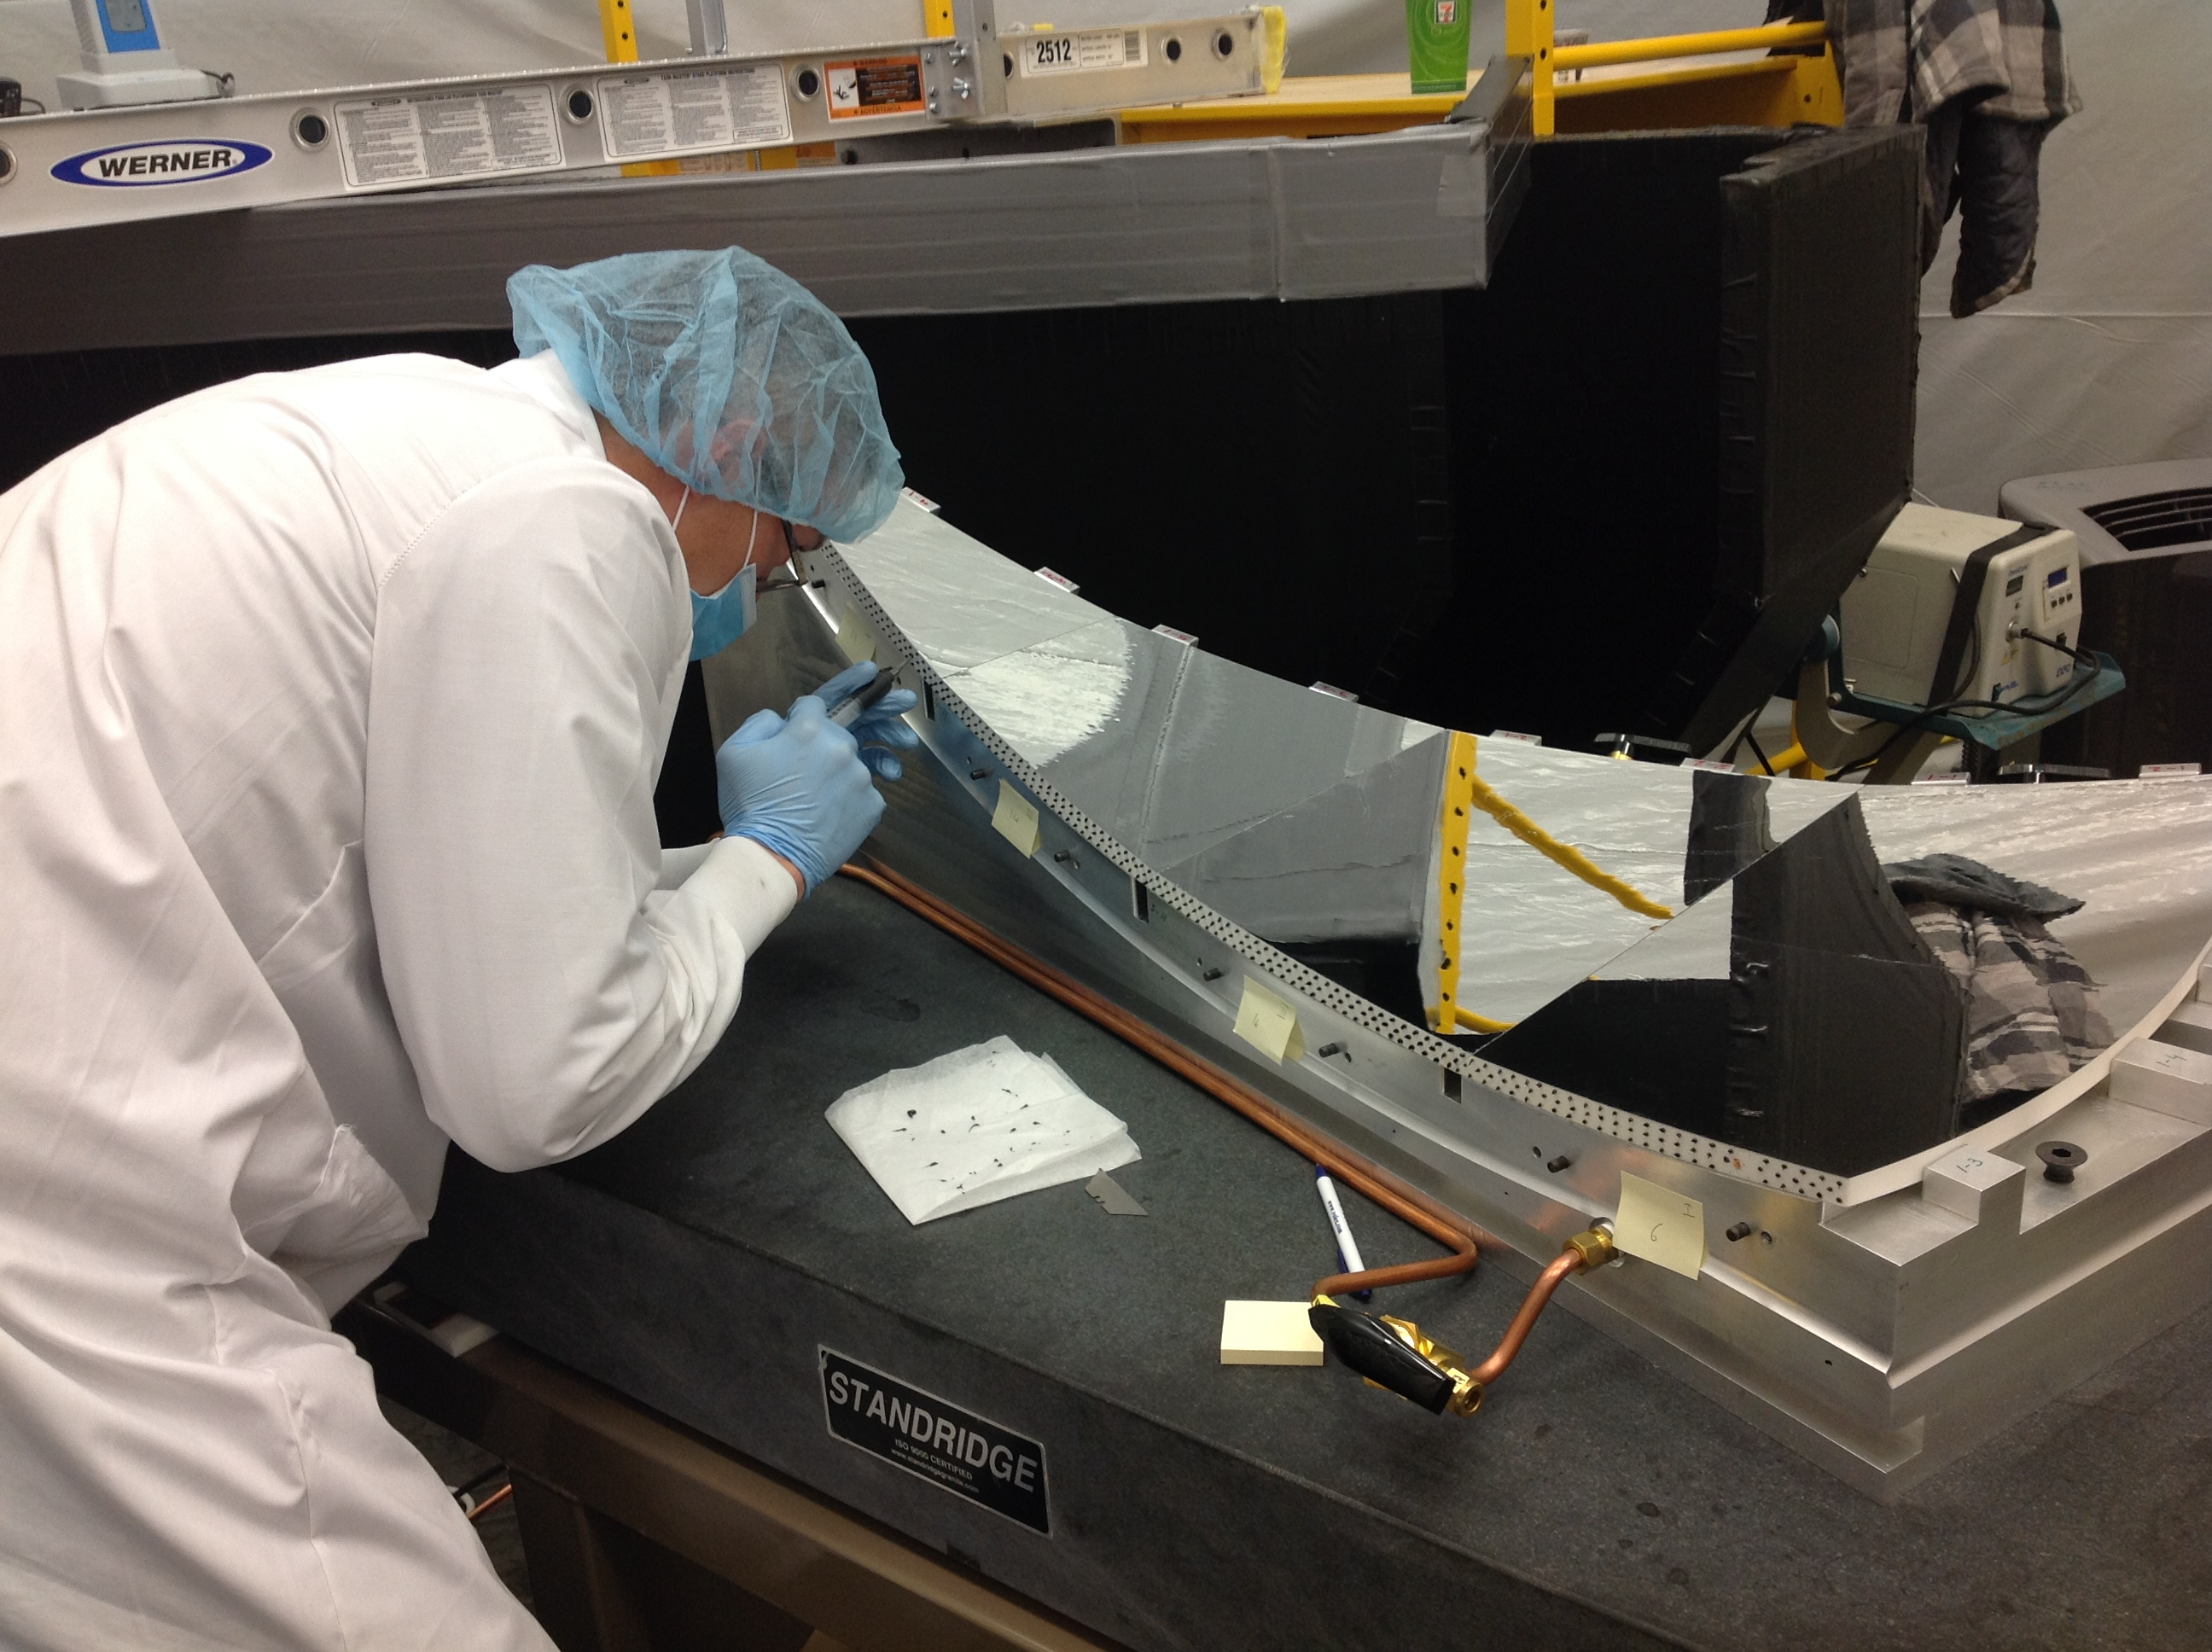
\includegraphics[trim={20cm 15cm 0 10cm },clip,width=\linewidth]{images/Picture3.JPG}
    \caption{Five ellipsoidal mirror facets glued together make up 1/12 of the HTCC mirror (half of the CLAS12 sector)}
    \label{fig:one_sector}
\end{figure}

\subsection {Ellipsoidal Mirror Facets Manufacturing}
\indent The usage of the high accuracy mechanical processing was absolutely unavoidable in providing an appropriate high precision mirror facets for the final combined mirror. Putting together 60 ellipsoidal facets of semi-trapezoidal shape fitting each other without adjustment of the overall dimensions of the adjacent facets seams to be not an easy task itself. In order to adjust the facets of the combined mirror each individual facet would need to have its own support infrastructure, and this would unavoidably introduce additional material. With these concerns in mind, all of the mechanical processing of the mirror facets was performed with a HAAS 5-axis milling machine. This allowed us to develop and use special trimming technology for the facets. One such technique was the "one shot" method, i.e. which provided the ability from one setting to trim any facet with 3 or 4 contact surfaces that needed to be glued. This was done to exclude, or at least minimize, the errors introduced when we reset the orientation of the facets while we cut 3 or 4 edge planes under different combine angles. We estimated that any deviation in the designed dimensions of more than about 0.005" would make the assembly of so many mirror substrates together impossible or, at the very least, difficult. This was because any post manufacturing adjustment of any of mirror substrates was not an option. In no way could facets be found to be either overlapping or with significant gaps. These gaps could be as wide as the thickness of a regular glue joint obtained by simple contact pressure. Otherwise, if these gaps were any larger, they would reduce the working acceptance and lead to additional inefficiencies that are harder to control or to fix.
\\
\indent Besides the polishing process of large mirrors (8-9 ft in diameter) usually means that the manufacturing of these mirrors is both labor intensive and time consuming, thus leading it to be very expensive. Therefore we have been looking for only radical solutions to completely avoid any polishing. Due to the fact that we did not require sharp images, the mirror facets were thus constructed to only work as efficient light collectors. To accomplish the goal we have developed and established entire assembly procedure following by tests the chain of construction and corresponding rating of final results.
\\
\indent Another issue we addressed was the choice between gluing or mechanical plug pin assembly procedures. Clearly gluing introduces deformations that are due to the shrinkage of any glue. On the other hand, an assembly procedure that uses location pins is a more complicated type of joint since it requires the high precision processing of plastic foam parts that are both very lightweight and mechanically weak. Moreover, if any joint deformation was observed after the first assembly attempt then many of the parts involved (including the mirror facets) could not be re-manufactured or used again.
\\
\indent We built 12 identical half-sectors of the combined mirror. All half-sectors consist of 4 ellipsoidal mirrors of different parameters. The outermost mirror was too large to trim it due to the limited travels of the milling machine table. Therefore this particular mirror was made of two mirrors being a mirror image of each other. Consequently in each half-sector was used 5 mirror substrates and the HTCC mirror consists of 60 ellipsoidal mirror facets in total. 

\indent All mirror facets have the same composite (sandwich) structure: Acrylic Film (thickness 0.010”) + Foam (thickness 0.600”) + Acrylic Film (thickness 0.010”). The mirror substrate was made from ROHACELL PMI (polymethacrylimide) foam. Acrylic films were of optical quality. they were covered with thin protection film. Manufacturing any substrate was a multistage process:
\begin{itemize}
    \item Thermal shaping of the acrylic film shells for the front (ellipsoidal) and back (spherical) of the mirror
    \item Manufacturing of foam substrates
    \item Assembly (gluing) of the sandwiched mirror substrate
    \item Trimming of the sandwiched mirror substrate
    \item Coating of the ellipsoidal faces of the substrate
    \item Reflectivity tests of the mirror substrate
    \end{itemize}

Correspondingly we used 5 different sets of high precision custom made tolling used for thermal shaping, gluing and trimming
the substrates. Thermal shaping was done in the low temperature PRECISION oven with less than  0.5$^\circ$C  temperature
uniformity in the volume. Set of tooling for the manufacturing of mirror facet \#2 covering polar angle in range of
$\vartheta = 12.5^\circ - 20^\circ$ and in azimuthal angular interval of $\Delta\varphi = 30^\circ$ is shown on Fig.\ref{fig:Tooling}.

\begin{figure}[h]
    \centering
    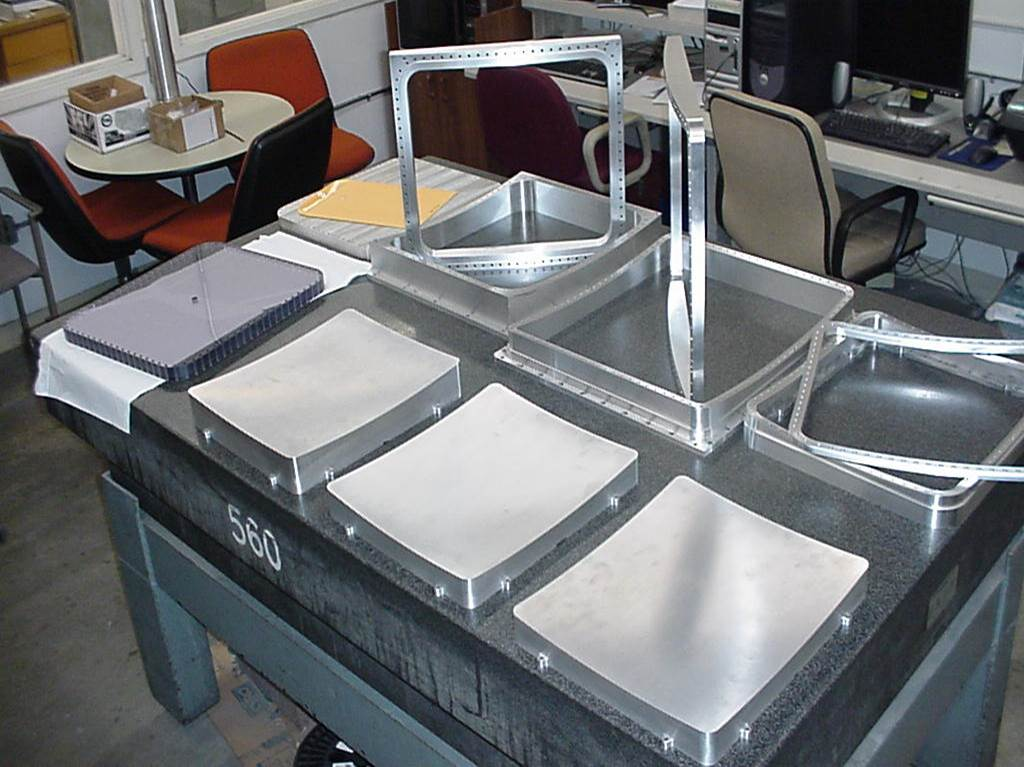
\includegraphics[width=1.0\linewidth]{images/Tool_on_tbl.jpg}
    \caption{Tooling set for the manufacture of mirror facet \#2}
    \label{fig:Tooling}
\end{figure}

\indent Scheme of shaping Acrylic shells is illustrated on the  Fig.\ref{fig:Shaping_new}. On the Fig.\ref{fig:Vac_Mol_Back}
is shown partially loaded tooling set for shaping back of the mirror in the oven. The shaping process was done at temperatures
about 105$^\circ$C and pressures bellow or about 1 ATM differential. We had two possibilities to shape shells: use vacuum shaping or just pressurizing the volume up to 2-3 psi differential. Since tooling parts were heavy the operations with oven would take about 3-4 hours. Whole process of shaping of one shell would take up to 5 hours.

\begin{figure}[h]
    \centering
    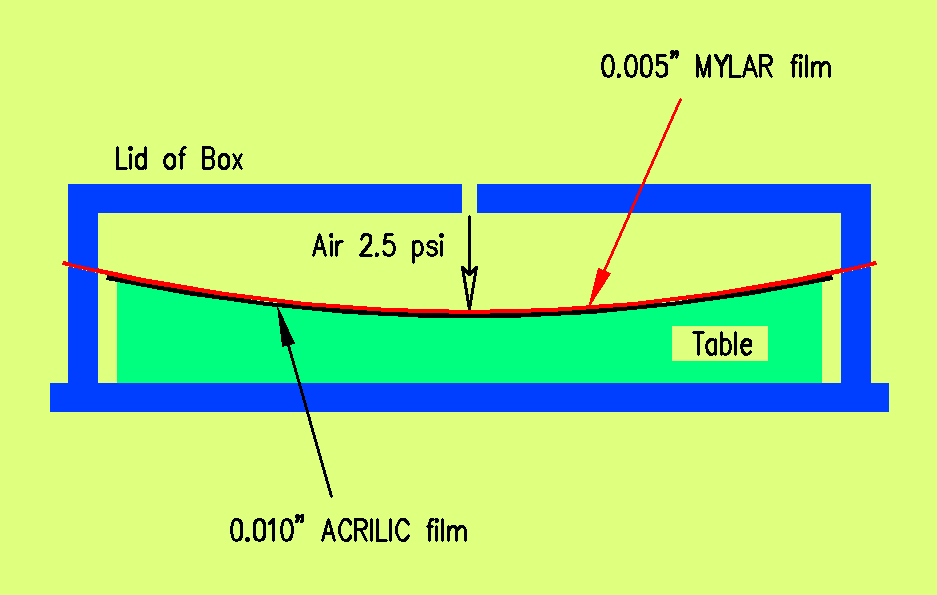
\includegraphics[width=1.0\linewidth]{images/Shaping_new.png}
    \caption{Scheme of thermal shaping of the spherical shell for back of the mirrors}
    \label{fig:Shaping_new}
\end{figure}

The loaded tooling set for the shaping the front ellipsoidal shell in the oven by pressurizing the volume above the film is shown on  Fig.\ref{fig:Pres_Shaping_Front}.

The next Fig.\ref{fig:Shell} shows the shaped acrylic shell for the front of the mirror.

\begin{figure}[h]
    \centering
    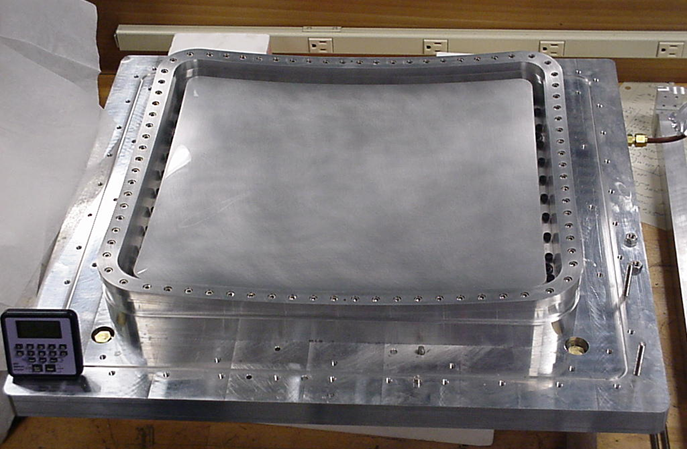
\includegraphics[width=0.95\linewidth]{images/Vac_Mol_Back.png}
    \caption{Partially loaded tooling set for shaping spherical back of the mirror facet \#2}
    \label{fig:Vac_Mol_Back}
\end{figure}

\begin{figure}[h]
    \centering
    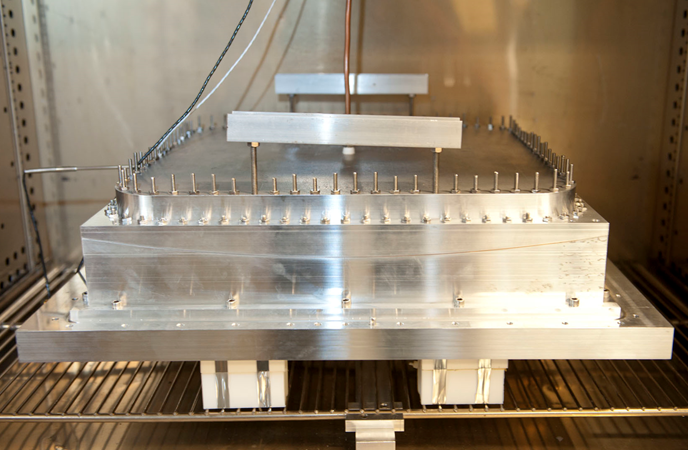
\includegraphics[width=0.95\linewidth]{images/Pres_Shaping_Front.png}
    \caption{Loaded tooling set for shaping front ellipsoidal shell of the mirror facet \#2 in the oven by pressurizing the volume}
    \label{fig:Pres_Shaping_Front}
\end{figure}

\begin{figure}[h]
    \centering
    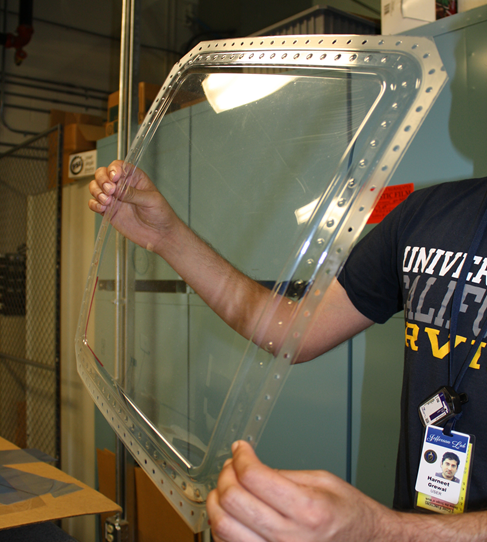
\includegraphics[width=0.90\linewidth]{images/Front_Shell.png}
    \caption{Thermally shaped front ellipsoidal shell for the mirror facet \#2}
    \label{fig:Shell}
\end{figure}

Preliminary cutout of the foam substrate and processing of its back surface of spherical shape was performed without using any custom made tools, see Fig.\ref{fig:Cut_Substr}.
\begin{figure}[h]
    \centering
    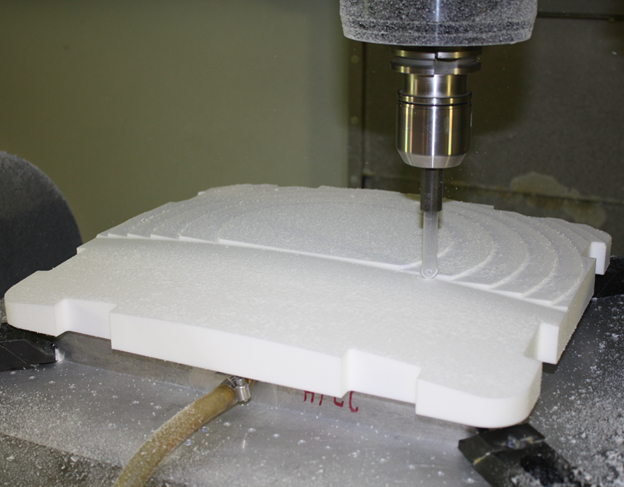
\includegraphics[width=0.9\linewidth]{images/Cut_Substr.png}
    \caption{Milling the back surface of the foam substrate \#2}
    \label{fig:Cut_Substr}
\end{figure}

The front ellipsoidal surface has been cut using the tooling that was also used for the final trimming of the sandwiched glued facet. Once the front surface was cut one had to take the facet off the used tooling set for the next operation of gluing Acryl-Foam-Acryl sandwich. On the Fig.\ref{fig:Foam_Sub} is shown the fully processed foam substrate \#2 ready for the assembly of the sandwich. 

\begin{figure}[h]
    \centering
    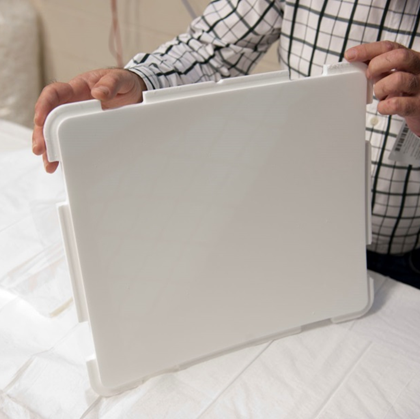
\includegraphics[width=0.9\linewidth]{images/Foam_Sub.png}
    \caption{Foam substrate is the core of the mirror facet}
    \label{fig:Foam_Sub}
\end{figure}

Scheme of assembly of the sandwiched substrate is brought on the Fig.\ref{fig:Gluing_Sandwich}.

\begin{figure}[h]
    \centering
    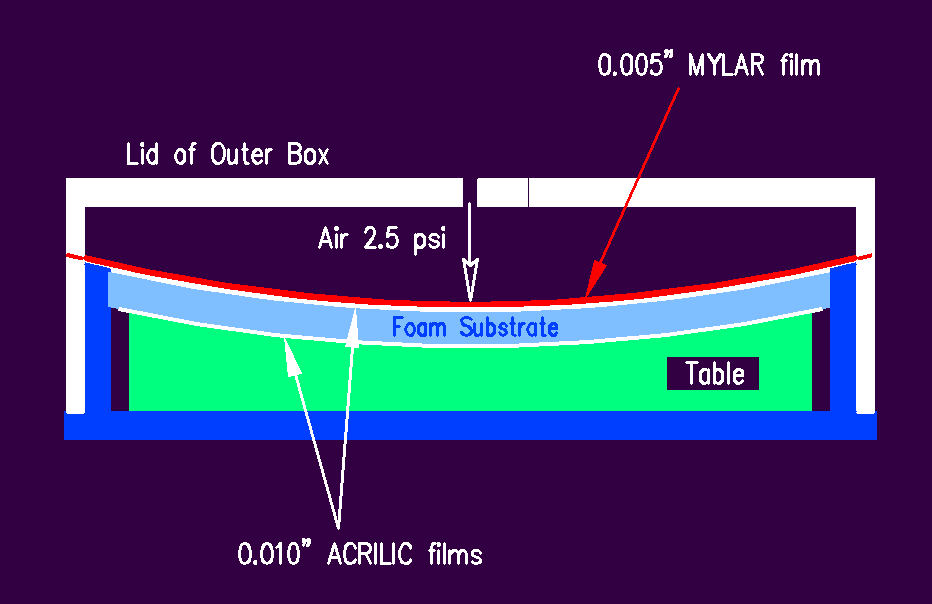
\includegraphics[width=0.9\linewidth]{images/Gluing_Sandwich_New.png}
    \caption{Scheme of gluing of sandwiched substrate}
    \label{fig:Gluing_Sandwich}
\end{figure}

On the Fig.\ref{fig:Assembled_Sandwich} one can see the fully assembled sandwiched substrate \#2 ready for the final trimming: 

\begin{figure}[h]
    \centering
    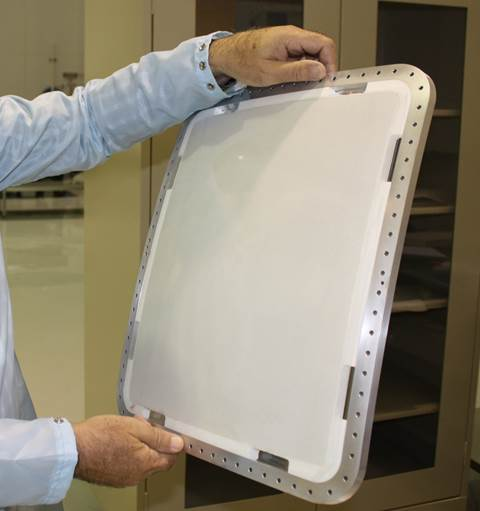
\includegraphics[width=0.9\linewidth]{images/Assembled_Sandwich.jpg}
    \caption{Sandwiched mirror facet after gluing components as shown in Fig.\ref{fig:Gluing_Sandwich}}
    \label{fig:Assembled_Sandwich}
\end{figure}

Then the sandwich was put back in the tooling set for the final precise trimming. The shells have been designed and processed in the way that allowed  unequivocal and simple alignment of all parts during assembly. Using the same set of tooling for cutting face and trimming the facet guaranteed automatic perfect relative alignment of the parts being glued together. Accuracy of alignment and therefore repeatability and reproducibility of results have been achieved. Before trimming operation the front working face of the substrate was covered with special tight-fitting protective film preventing damage or pollution of the working surface while trimming the substrate. For better control the first manufactured mirror facets have been assembled using epoxy glue with black dye. Trimming was done in two steps. In order to avoid shell pealing off the foam the foam substrate the shell was cut through using very small diameter end mill, see Fig.\ref{fig:Trimming_1}:

\begin{figure}[h]
    \centering
    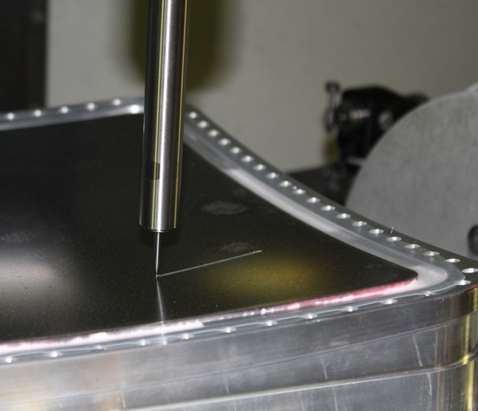
\includegraphics[width=1.0\linewidth]{images/Trimming_1}
    \caption{Cutting through the acrylic shell of the substrate using small diameter end mill}
    \label{fig:Trimming_1}
\end{figure}

Then the outer portion of the shell was safely pealed off the substrate and then trimming was performed using long enough end mill. The completed final trimming of the facet is show on the next Fig.\ref{fig:Trimming_2}.

\begin{figure}[h]
    \centering
    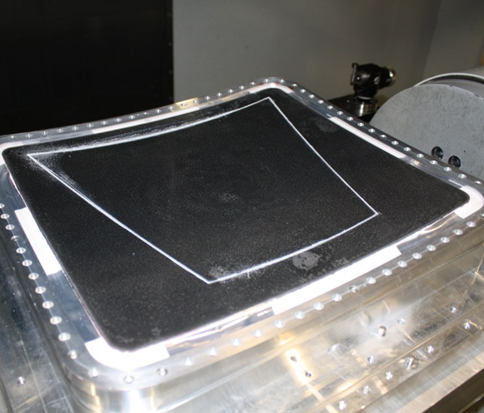
\includegraphics[width=1.0\linewidth]{images/Trimming_2}
    \caption{Completed final trimming of the mirror facet \#2}
    \label{fig:Trimming_2}
\end{figure}

During final milling the substrate has been secured in place by inserting soft foam wedges along partially cut sides and glued to the outer portion of the substrate being trimmed. This completely eliminated any vibration that usually ruins accuracy of processing. On the  Fig.\ref{fig:Trimmed} is shown completed mirror facet \#2 ready for deposition of reflective coating. All trimming has been done from one setting, i.e.without any re-positioning of the facet. 

\begin{figure}[h]
    \centering
    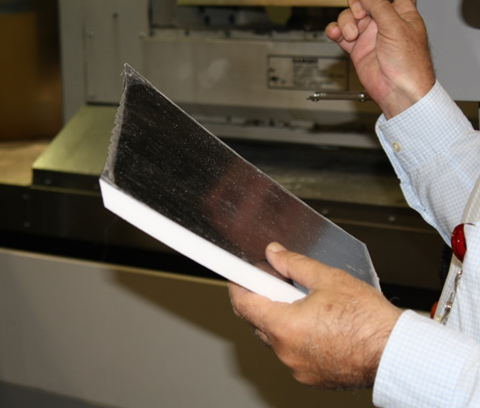
\includegraphics[width=1.0\linewidth]{images/Trimmed}
    \caption{Completely trimmed mirror facet \#2 covered with protection film }
    \label{fig:Trimmed}
\end{figure}

The face of the mirror substrate did not require any processing before deposition of a reflector material. The total thickness of the mirror is 130-135 mg/$cm^{2}$. The acrylic films were glued to both sides of the substrates to compensate deformation introduced by shrinking thin epoxy glue layers as a result of polarization. No shrinkage effects observed thus the long term problems with mirror shape was completely eliminated. All critical mirror fabrication steps have been performed in the Clean Room (Class 1000). In addition for better results all parts have been individually cleaned using ionizing gun right before assembly. Besides in the clean room right next to the assembly table the was installed clean bench with HEPA air filter that was blowing filtered air over the table. Thermal and mechanical processing was done either with protection films covering critical surfaces or encapsulated in the gas tight volume. This was to prevent dust and any other unwanted depositions from damaging the working surface or otherwise compromising the mirror reflectance.

\subsection{Tests of Mirrors Coated with Reflective Material}
Evaporated Coatings Incorporated (ECI) was chosen from among four potential vendor companies to perform vacuum deposition of the reflective coating onto the HTCC Mirror Substrates.The test samples (flat sheets of Acryl, one untouched and one subjected to the same thermal shaping process used to form the front and back surfaces of the mirrors) coated by ECI were the most reflective over the entire wavelength range of interest. A 30 W Deuterium lamp was used as a UV source from 200-400 nm, and a 50 W quartz-tungsten halogen (QTH) lamp was used as a source of visible light from 370-650 nm. The monochromatic test beam for the reflectivity measurements was generated by a Newport model 74125 computer-controlled monochromator. A Newport model 10Z40Al.2 flat broadband mirror was used as a repeatable reference standard for reflectance measurements. The mirror consists of a UV-enhanced aluminum coating on a 6 mm- thick, 1"-diameter Zerodur substrate, with a protective overcoat of UV-transparent Magnesium Fluoride to prevent oxidation.
The custom coating material used by ECI has acceptable reflection coefficient in UV-range and is resistant to oxidation at room temperatures. Each mirror facet has been coated individually and then tested at the company.  Input control of quality of the coated mirror facets has been done at Jefferson Lab. On the Fig.\ref{fig:JLab_Mirror}  are shown typical results of reflectance  measurements of ellipsoidal mirror facet for the HTCC.

\begin{figure}[h]
    \centering
    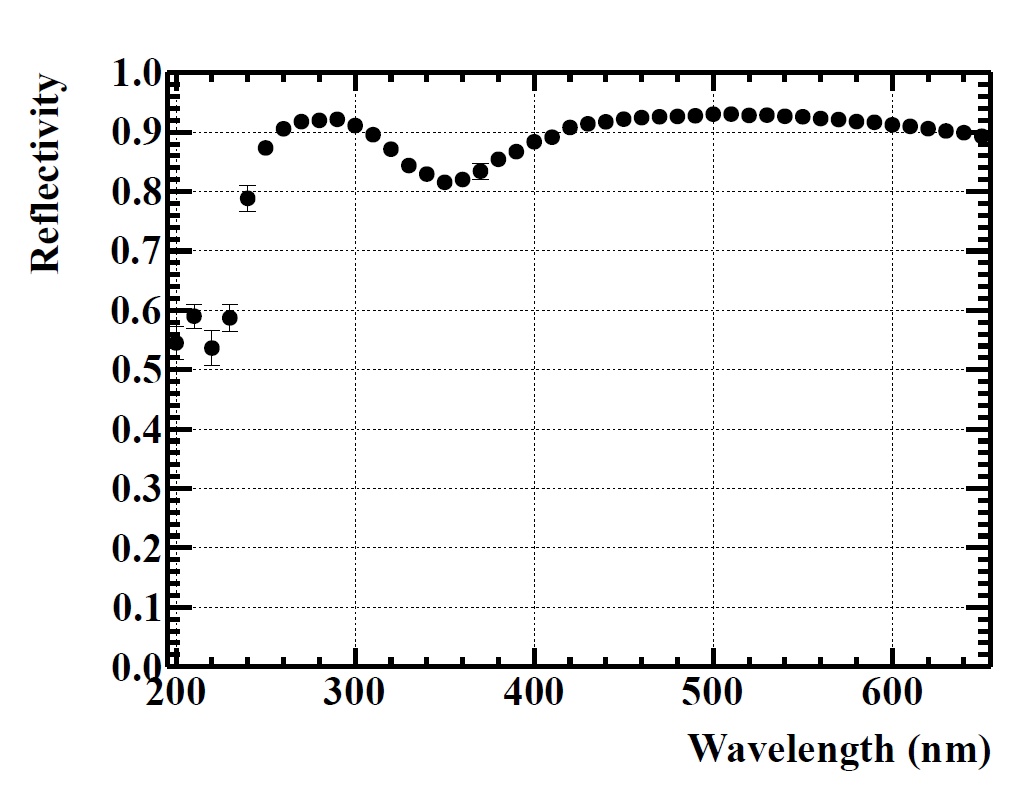
\includegraphics[width=1.0\linewidth]{images/JLab_Mirror}
    \caption{Typical reflectivity of the ellipsoidal mirror facet as measured at JLab}
    \label{fig:JLab_Mirror}
\end{figure}

The reflectance of the reference flat 1"-diameter mirror specified by vendor and checked at Jlab is brought on the Fig.\ref{fig:Ref_Mirror}. 

\begin{figure}[h]
    \centering
    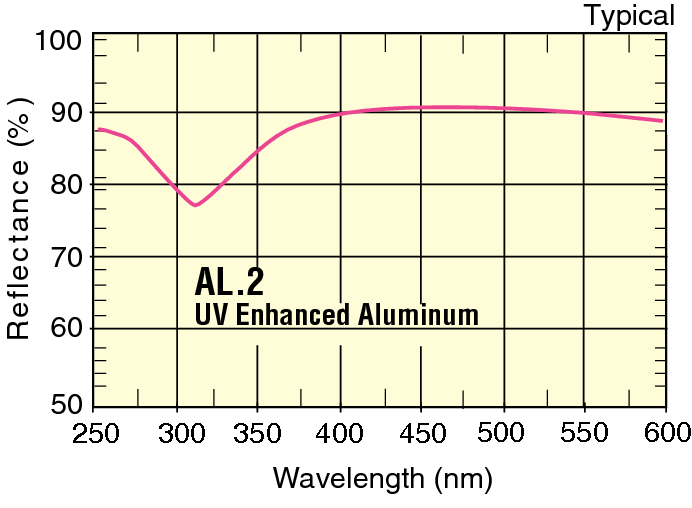
\includegraphics[width=1.0\linewidth]{images/Ref_Mirror}
    \caption{Typical mirror as specified by Newport}
    \label{fig:Ref_Mirror}
\end{figure}

The measurement technique has small systematic uncertainties of about 1-2\%. 
% has metallic Aluminum coating protected by Aluminum Fluoride (&AlF$_3$) layer. On the same picture are shown results on reflectance of the "witness piece" provided by ECI.

\subsection{Assembly and Tests of Half-sector Mirrors}
The assembly of the Half-sector mirrors have been performed on the high precision Half-sector assembly table. We had to guarantee usage of such assembly procedure that would eliminate Half-sector overlaps or having big gaps between them. On the Fig.\ref{fig:Half-sector_assem_tb2} is shown the table used in assembly of all 12 Half-sector mirrors. The table was made of solid Aluminum alloy block and has several features important for assembly of required accuracy:
\begin{itemize}
    \item Overall dimensions of the working surface was defining overall dimensions of the Half-sector mirror being assembled 
    \item The table was equipped with side plates from left and right of each facet (8 plates total)
    \item The table can be used for assembly by gluing facets to each other or assembly using location pins
    \item Radial and transverse position of the mirror could be controlled with accuracy up to 0.001" inserting spacers between mirror and the side plates
    \item Each of 5 places for mounting 5 different mirror substrates were working as a vacuum table of spherical work surface, i.e. each  facet used in assembly could  be put on the table and then secure in the place as needed by turning on the corresponding  diaphragm vacuum pump
    \item Along edges of the adjacent mirrors that are in contact the table has milled out groves for collecting excessed epoxy glue to prevent gluing of the facet to the table surface
    \item Polymerization of epoxy glue was possible to perform in the temperature and humidity controlled ambient   
    \item The table was a part of the setup allowing geometry tests of the assembled Half-sector
\end{itemize}

\begin{figure}[h]
    \centering
    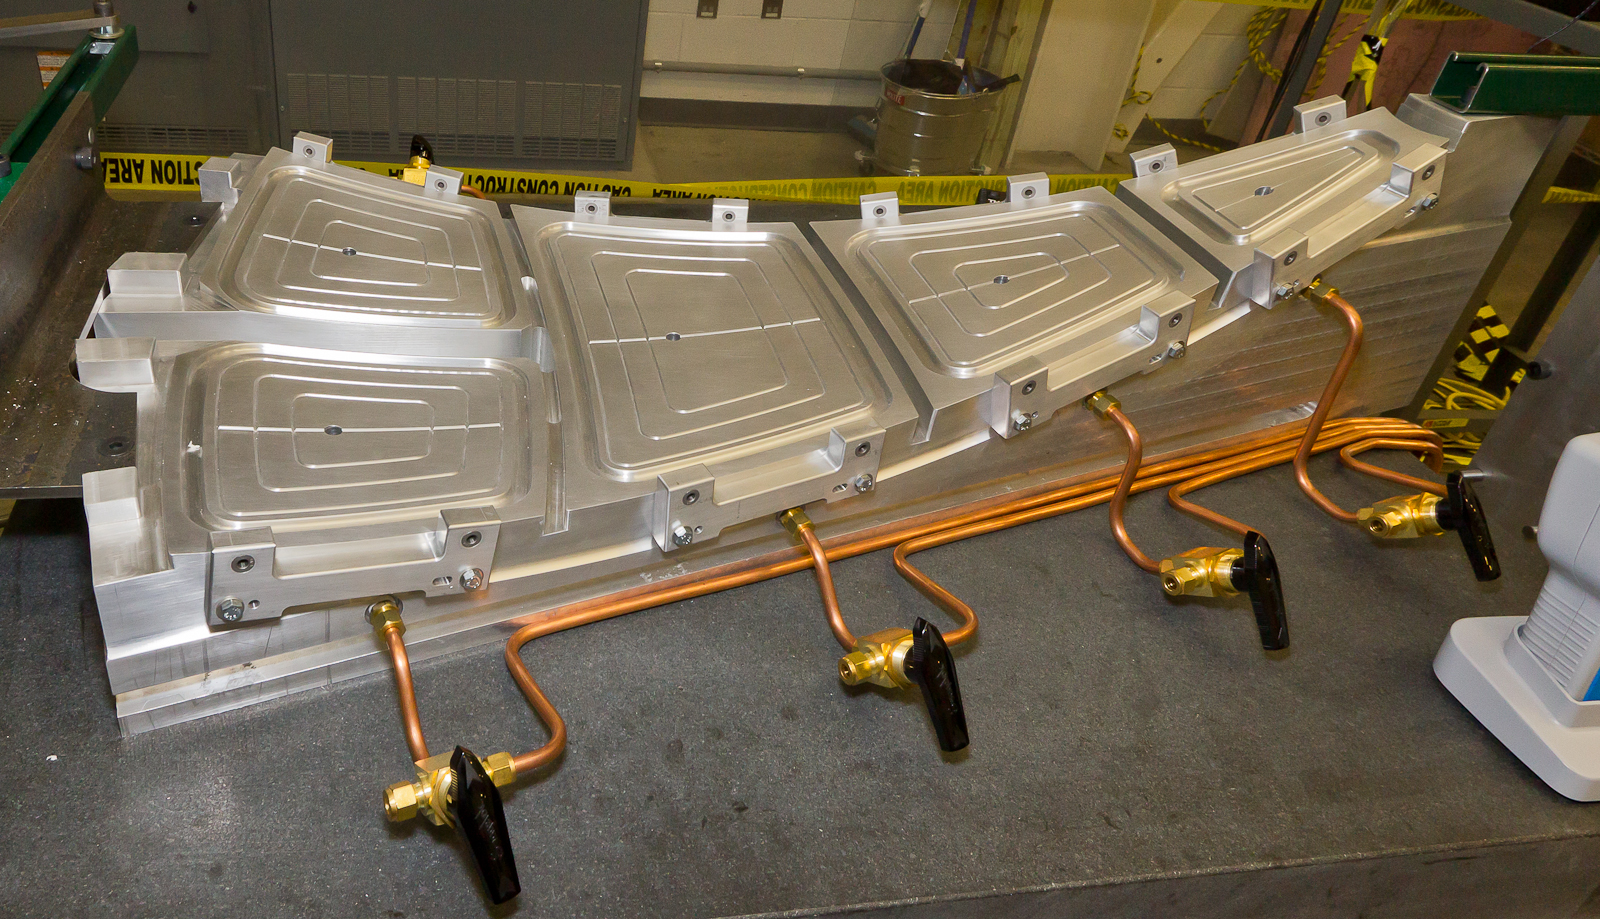
\includegraphics[width=1.0\linewidth]{images/Half-sector_assem_tb2.JPG}
    \caption{High precision table for assembly of the half-sector mirrors}
    \label{fig:Half-sector_assem_tb2}
\end{figure}

\indent Assembly of the combined mirror using location pins is preferable as compared with side-to side direct gluing there are no deformations involved due to unavoidable epoxy glue shrinkage. Nevertheless it has been decided not to use location pins since the thickness of the substrates (0.6") was relatively small and the mechanical strength of the PMI foam that we used would introduce risks during final assembly of the HTCC mirror, its handling and installation. Therefore we decided to directly glue the facets to each other but using simple technique of gluing. Namely we were applying the glue in form of glue dots uniformly distributed over contact surface. Amount of glue in dots and distance between them were such that the spots  of humps of glue smashed between facets were not touching each other. In this case deformations caused by shrinkage of individual dots cancel each other and the shape of the final product stays unchanged. The only dots that introduce not compensated shrinkage deformation are near the edges of the glued surfaces. Corresponding deformations does not change mirror shape but they introduce slight residual waviness of the edges of the mirrors. Waviness pattern repeats an actual pattern of dots along the edges. In fact the only concern was to make sure the glue joints are strong enough. We run comprehensive tests to come up with acceptable solution for using this kind of joints. We  tried several different patterns of glue application, amount and viscosity of glue, applying glue on side or both sides.
On the Fig.\ref{fig:Pattern} are shown two identical foam pieces and epoxy application pattern used in the tests of glue joint. 

\begin{figure}[h]
    \centering
    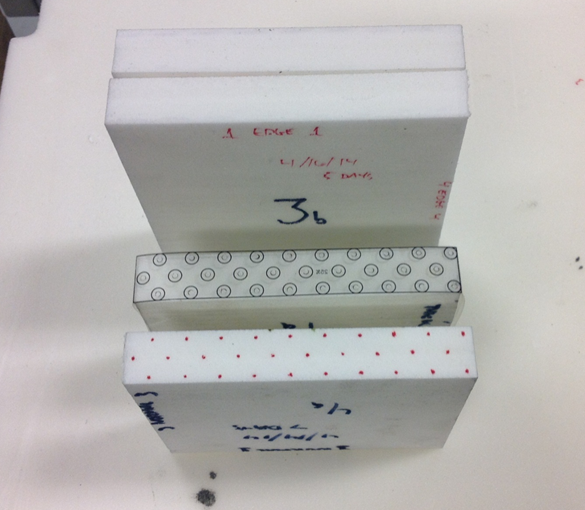
\includegraphics[width=1.0\linewidth]{images/Pattern.png}
    \caption{Foam pieces marked for approximately 22.5\% epoxy coverage pattern}
    \label{fig:Pattern}
\end{figure}

Standard Hysol Epoxy with black pigment and 1:1 \% Silica filler to epoxy by volume were applied as small dots (0.08 inch of diameter).The viscosity of the epoxy filler mix was so thick that none of the glue bleed across the foam occurred. After the two test parts epoxy joint had cured the parts were then glued to two aluminum test blocks, see Fig.\ref{fig:Glue_joint_test}.

\begin{figure}[h]
    \centering
    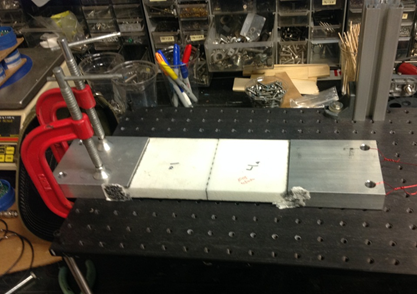
\includegraphics[width=0.95\linewidth]{images/Glue_joint_test.png}
    \caption{Test setup to check strength if the glue joint}
    \label{fig:Glue_joint_test}
\end{figure}

Parts were allowed to cure for an additional 72 hours. Results of tests are shown on Fig.\ref{fig:Broken}. 

\begin{figure}[h]
    \centering
    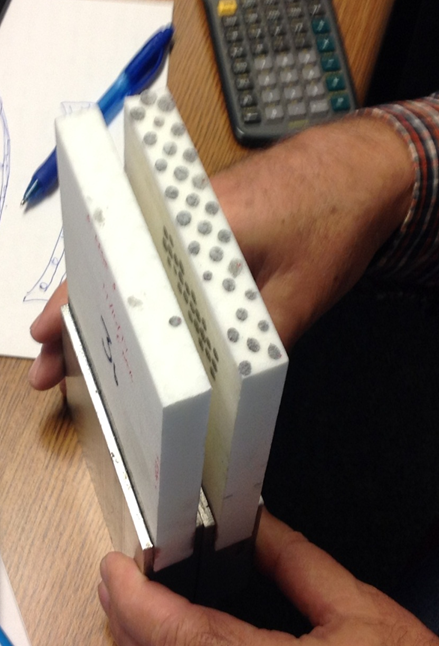
\includegraphics[width=1.0\linewidth]{images/Broken.png}
    \caption{Broken epoxy glue joint between two PMI foam pieces}
    \label{fig:Broken}
\end{figure}

Total force to break the glue joint  was about 62 ft. lbs. The force was applied very evenly and the foam was torn from the glue on both test pieces. The foam failed not the glue itself. There was set a 0.004 inch wide gap left between parts when gluing. The glue was directly applied to one piece only. Yet it still made a terrific bond able to pull out almost all of the glued dots evenly except for the two places where the shims were set. One foam piece which has the dots on it, is the same piece the epoxy was applied to.

It has to be mentioned that the glue dots applied along the sides of the adjacent mirror facets very will compensate the shrinkage of each other that occurs after polymerization of epoxy is completed. There are only two not compensated dots at the ends of any side to be glued. The effect of the shrinkage is too small because all other dots along the glued sides are properly compensated and therefore shape of the facet stays unchanged. Since along sides of any glued facets there are 3 to 4 rows of applied glue dots. Than the dots across the width of the glued side are mostly not compensated. This directly leads to a certain deformation of edges of the glued facets, i.e. the edge is still smooth line  but "wavy" and waviness pitch is defined by average distance between adjacent glue dots. In other words the local light collection efficiency of the mirror facets along glued sides only decreases since geometry of the edges are changed. It was possible to avoid this small decrease if more complicated joint with location pins was used. Corresponding results obtained in the experiments with electron beam will yet be discussed.

The high precision table was part of the the half-sector mirror geometry tests setup. The setup was equipped with low energy red laser gimbal mounted in the target position and with four focal planes. Relative location of the laser, assembly table and focal planes were strictly defined by designed geometry of the HTCC light collection. The setup allowed check actual geometry of light collection by each mirror using point-like laser beam as well as the beam rastered in the plane crossing any mirror over its entire surface. The assembly of half-sectors was done step by step by placing on the table mirror facets starting from the smallest mirror. The first facet once placed on the table was aligned and then checked whether it fits to the place and provides designed gaps between both sides and the side plates from left and right. After that the vacuum pump was turned on to secure the mirror in the right place. It was impossible to shift the facet sucked to the table by even a little bit without deforming the mirror. Than the adjacent mirror with epoxy glue dots on it was placed next providing contact with the first mirror. Once aligned it was independently secured on the table using same vacuum pump. Epoxy glue dots was applied on the every next following facet and procedure was repeated until half-sector was assembled. On the Fig.\ref{fig:Partial_Half-sector} is shown partially assembled half-sector mirror. The right half (installed) and left half (yet missing) of the largest mirror have exactly the same geometry. 

\begin{figure}[h]
    \centering
    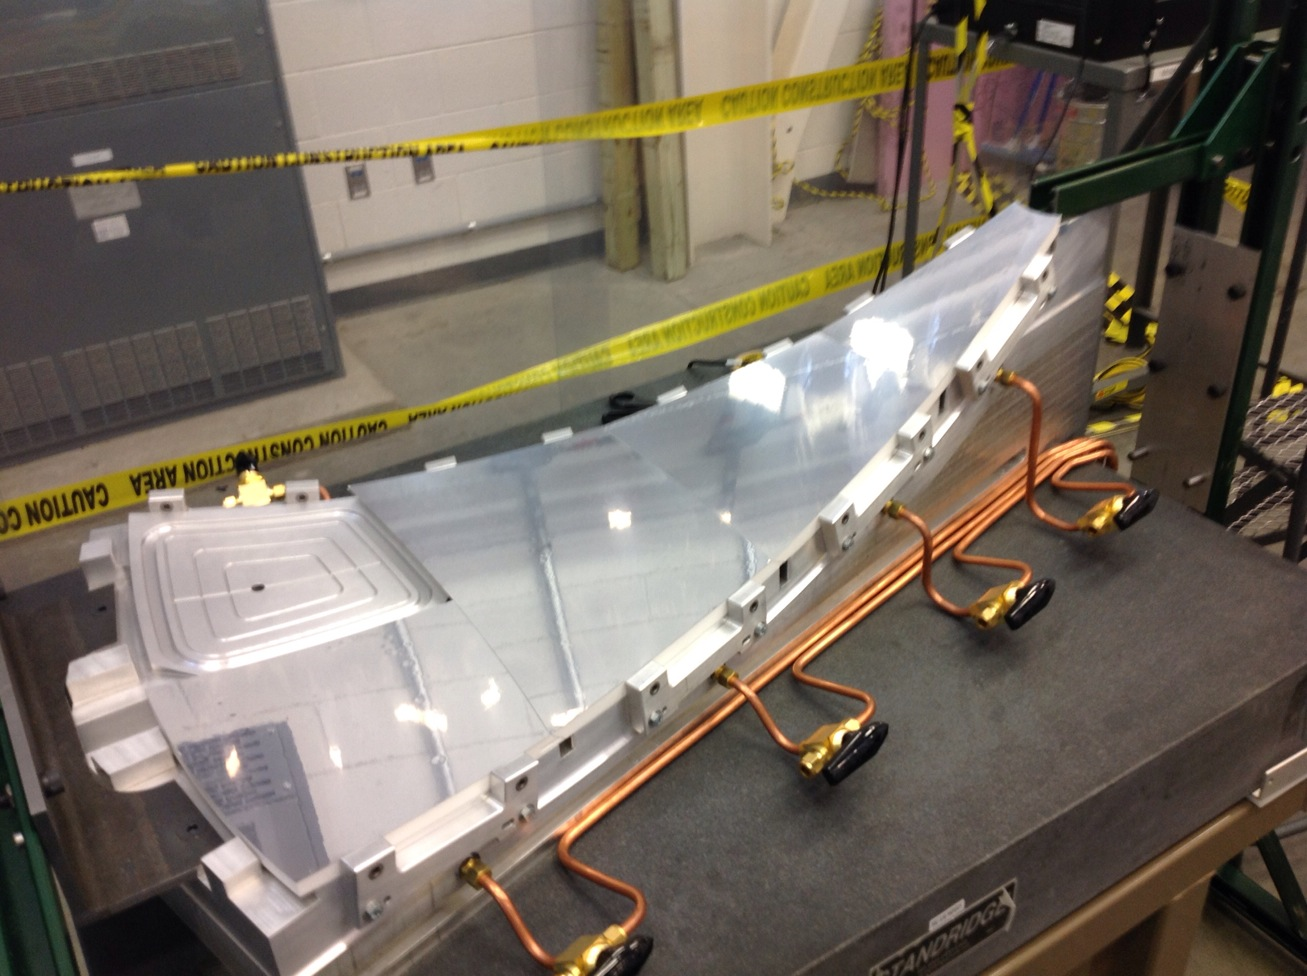
\includegraphics[width=1.0\linewidth]{images/Partial_Half-sector.png}
    \caption{Partially assembled half-sector mirror. Left facet of the last largest mirror is not installed yet}
    \label{fig:Partial_Half-sector}
\end{figure} 
On the Fig.\ref{fig:Half-sector} is shown fully assembled half-sector mirror. It was left on the table under the pressure with vacuum pumps on for at least 24 hours or more depending on polymerization results of the control glued samples. 

\begin{figure}[h]
    \centering
    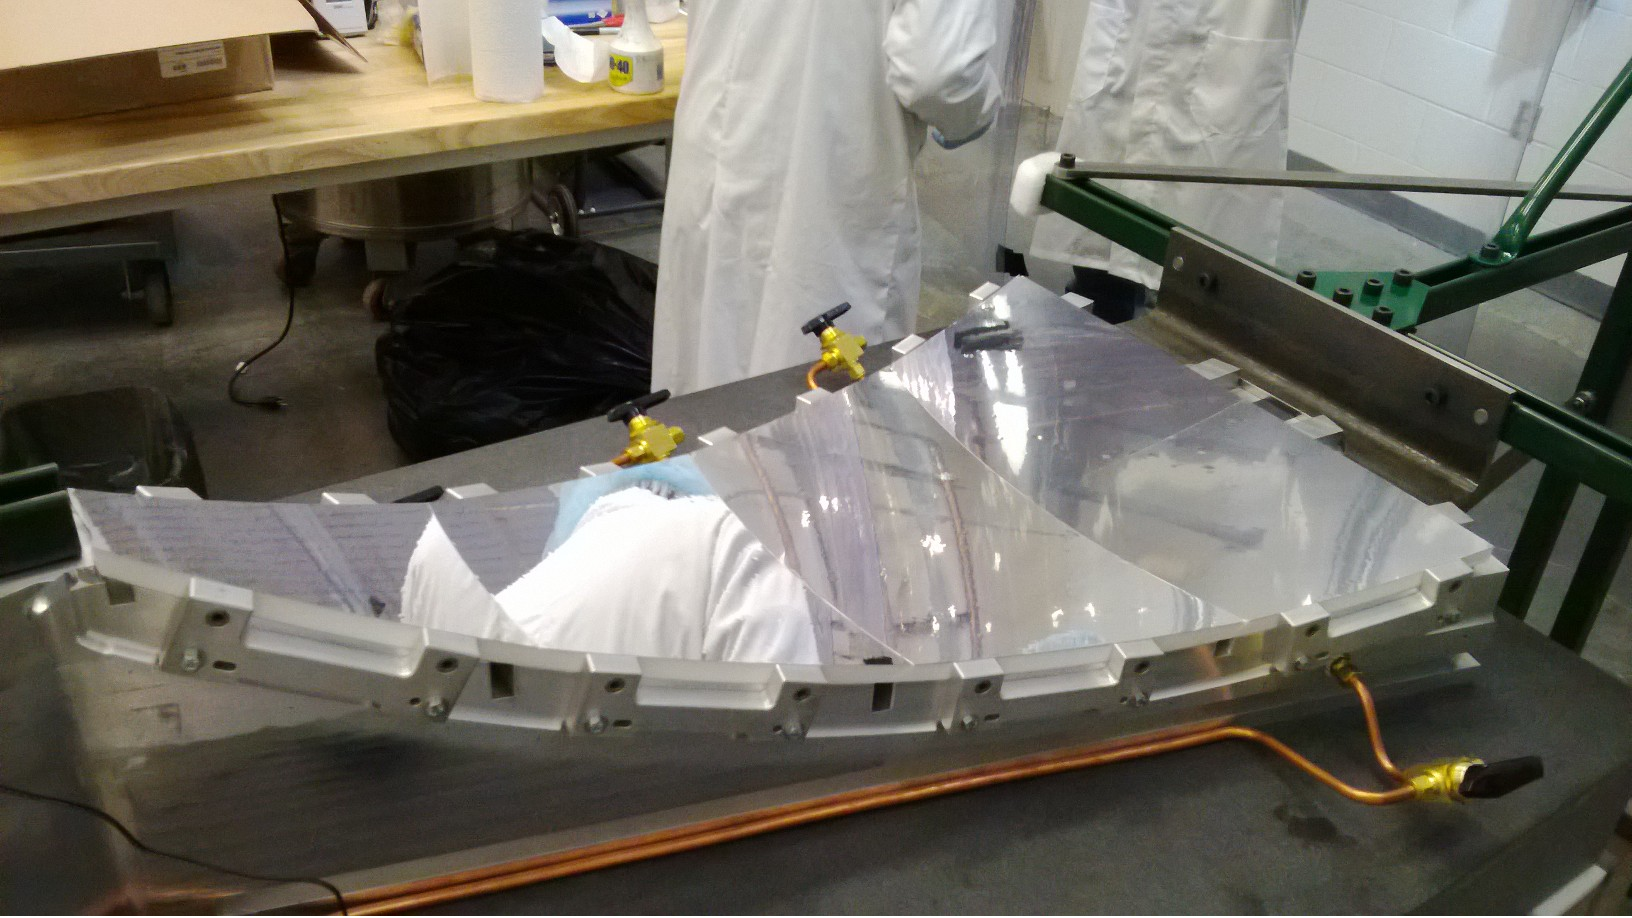
\includegraphics[width=1.0\linewidth]{images/Half-sector.png}
    \caption{Fully assembled half-sector mirror. The largest mirror consist of two mirror facets which have the same geometry}
    \label{fig:Half-sector}
\end{figure}

\indent Light collection geometry was checked on the half-sector mirror geometry tests setup after complete polymerization of the glue. Obtained Pattern of the light collection obtained on the focal plane of the smallest mirror facet that is covering polar and azimuthal angles of scattering electrons in the range of $\vartheta = 5^\circ - 12.5^\circ$\, and\, $\varphi = 0^\circ - 30^\circ$ is shown on the Fig.\ref{fig:Focal_Plane_4}. The the concentric circles on the focal plane are of diameter 1, 2 and 3 inches.  

\begin{figure}[h]
    \centering
    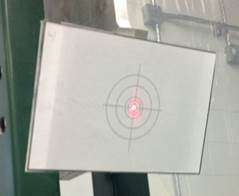
\includegraphics[width=0.90\linewidth]{images/Focal_Plane_4.jpg}
    \caption{Light collection pattern on the focal plane. Laser beam is rasterized in the plane crossing the mirror covering polar and azimuthal angles in the range of $\vartheta = 5^\circ - 12.5^\circ$\, and\, $\varphi = 0^\circ - 30^\circ$}
    \label{fig:Focal_Plane_4}
\end{figure}

Similar results have been obtained for the remaining three mirror facets covering polar angular range of $\vartheta = 12.5^\circ - 20^\circ$,\, $\vartheta = 20^\circ - 27.5^\circ$,\, and $\vartheta = 27.5^\circ - 35^\circ$\, correspondingly. The azimuthal angular range is of\, $\varphi = 0^\circ - 30^\circ$\, for all mirror facets, see Fig.\ref{fig:Focal_Plane_3}, Fig.\ref{fig:Focal_Plane_2}, and Fig.\ref{fig:Focal_Plane_1R}.

\begin{figure}[h]
    \centering
    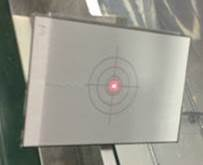
\includegraphics[width=0.90\linewidth]{images/Focal_Plane_3.jpg}
    \caption{Light collection pattern on the focal plane for the mirror covering polar and azimuthal angles in the range of $\vartheta = 12.5^\circ - 20^\circ$\, and\, $\varphi = 0^\circ - 30^\circ$}
    \label{fig:Focal_Plane_3}
\end{figure}

\begin{figure}[h]
    \centering
    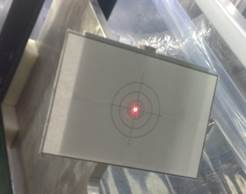
\includegraphics[width=0.94\linewidth]{images/Focal_Plane_2.jpg}
    \caption{Light collection pattern on the focal plane for the mirror covering polar and azimuthal angles in the range of $\vartheta = 20^\circ - 27.5^\circ$\, and\, $\varphi = 0^\circ - 30^\circ$}
    \label{fig:Focal_Plane_2}
\end{figure}

\begin{figure}[h]
    \centering
    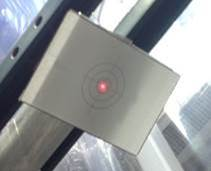
\includegraphics[width=0.95\linewidth]{images/Focal_Plane_1R.jpg}
    \caption{Light collection pattern on the focal plane for the mirror covering polar and azimuthal angles in the range of $\vartheta = 27.5^\circ - 35^\circ$\, and\, $\varphi = 0^\circ - 30^\circ$}
    \label{fig:Focal_Plane_1R}
\end{figure}

\indent All 12 half-sector mirrors have been assembled following exactly the same procedures that allowed us to control closely the overall dimensions and therefore defining ranges for values of the gaps between adjacent half-sectors. 

\subsection{Assembly of the HTCC Combined Mirror}

 The HTCC combined mirror has been assembled based on the experience acquired during half-sectors final assembly. In order to do this we have designed and build the vacuum half-sector mirror holding table for assembly of the combined mirror. The design of this table and accuracy of manufacturing and construction were critical in providing the required parameters of the combined mirror such as the geometry of the mirror optics, stability of its shape and mechanical integrity. Peculiar feature of the HTCC combined mirror is that the installed combined mirror had to provide correct light collection geometry for its all 60 mirror facets glued together. The option of having a possibility of any even very small adjustments of individual facets was excluded.
 
 \indent In fact we had to build 12 identical half-sector assembly tables and put them together due to relatively large overall dimensions of the HTCC mirror. The only difference between the high accuracy half-sector assembly table and 12 identical tables for the final assembly was that they did not have the side plates. On the Fig.\ref{fig:One_Foam_Vacuum_Table} is shown one of 12 such vacuum tables made of medium density Polyurethane foam with 100\% closed cells.
 
\begin{figure}[h]
    \centering
    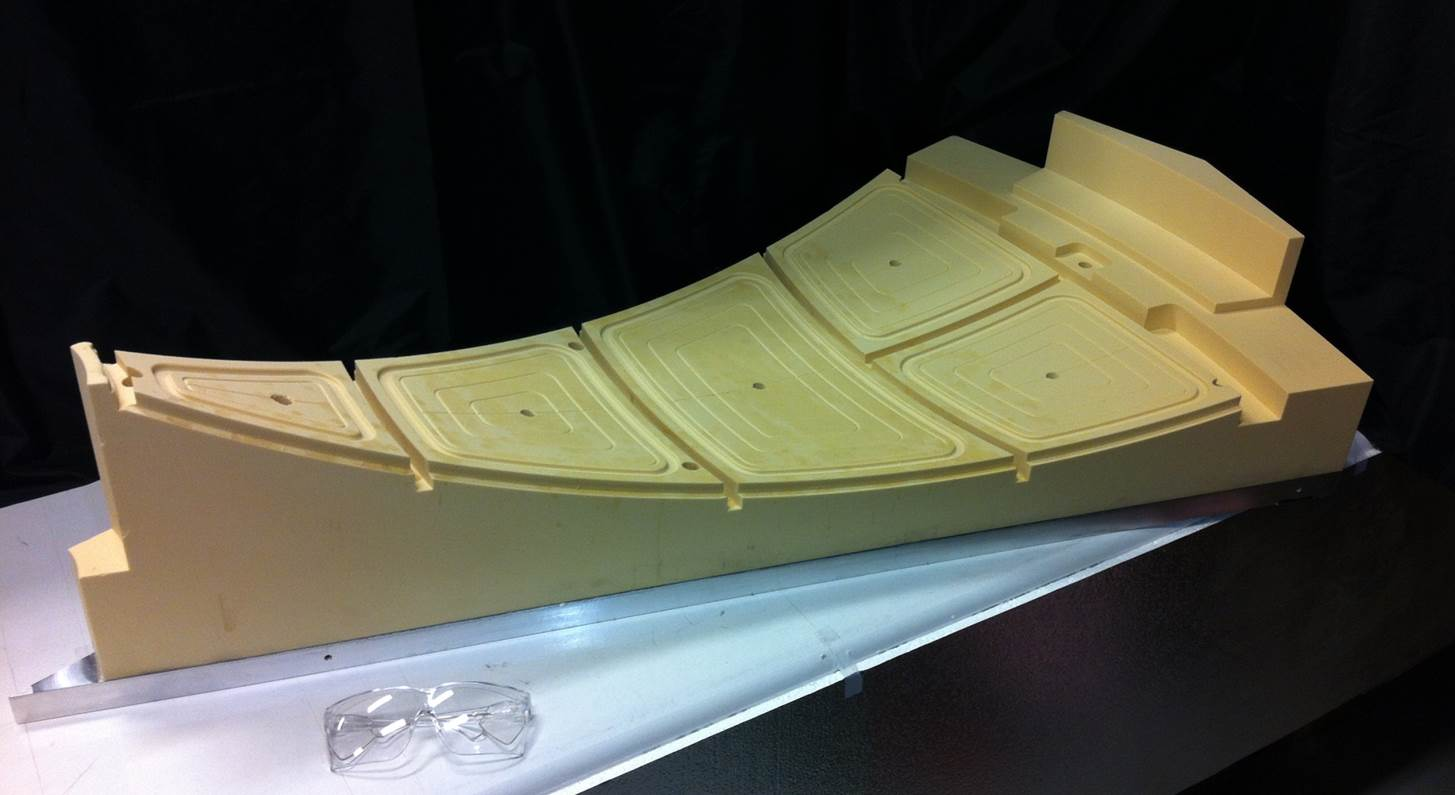
\includegraphics[width=1.0\linewidth]{images/One_Foam_Vacuum_Table.jpg}
    \caption{One of the 12 Polyurethane half-sector holding tables}
    \label{fig:One_Foam_Vacuum_Table}
\end{figure}
 
\indent The top portion of the table is made of one solid block of polyurethane foam. It is glued to the aluminum wedge-shaped flat plate 1 inch thick. To avoid or minimize possible warping we used plates of 1100 aluminum alloy. The smoothness and accuracy of manufacturing the top surface of the table were high enough to ensure the ability of the table to firmly hold the half-sector mirror. No gaskets of any kind were used to enhance the holding ability of the table. On the working surface of the vacuum table there are five circular, not interconnected grooves through which individually and independently air is pumped out under each of the five mirror facets of which the half-sector mirror consists.
\\
\indent The entire set of 12 half-sector vacuum holding tables was assembled on two identical flat plates 1 inch thick carrying 6 tables each. Six vacuum foam tables fully assembled on one of identical 1 inch plates are shown on the Fig.\ref{fig:Six_Foam_Vacuum_Tables}.
 
\begin{figure}[h]
    \centering
    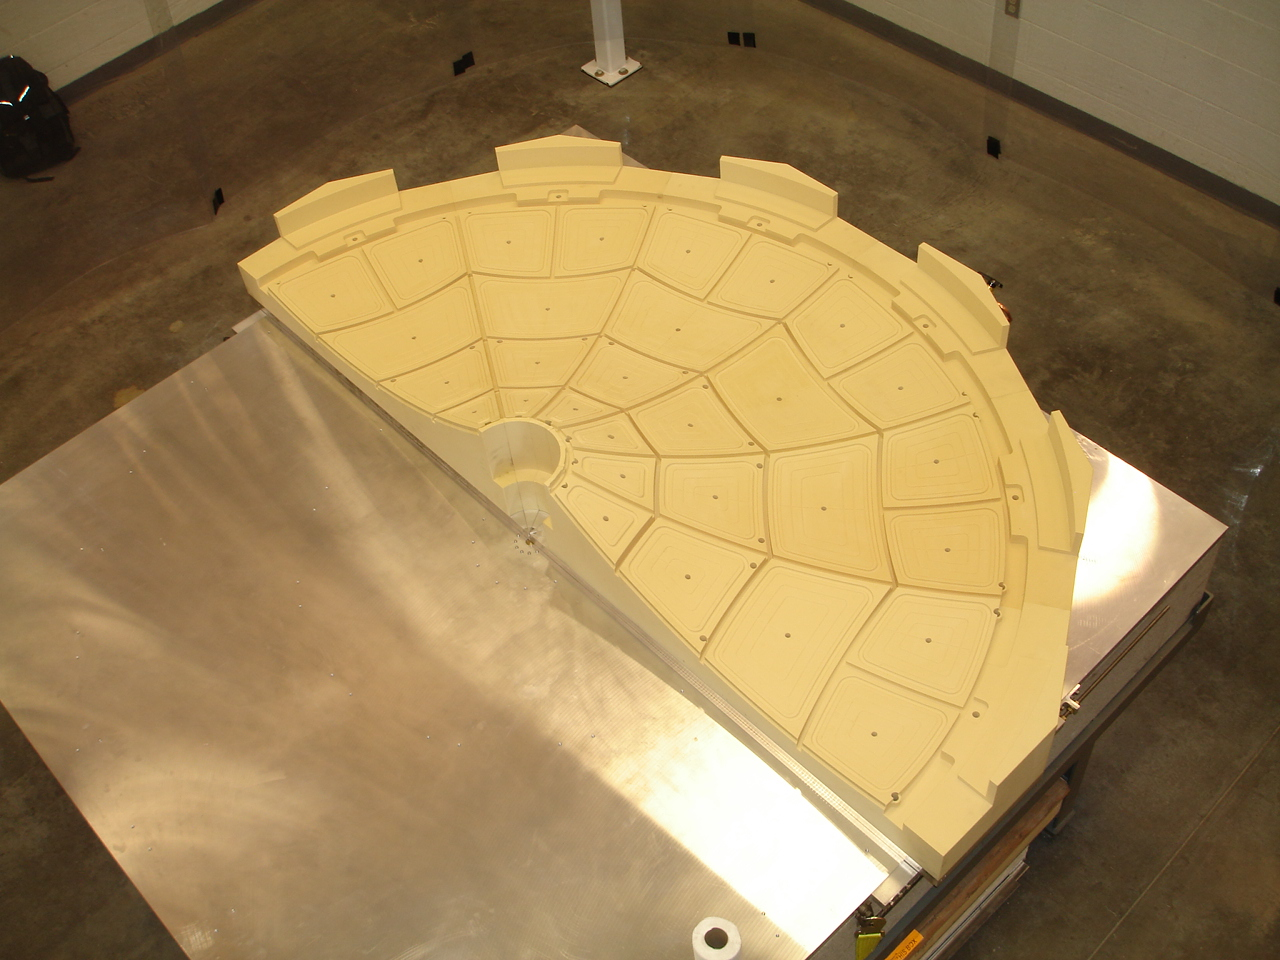
\includegraphics[width=1.0\linewidth]{images/Six_Foam_Vacuum_Tables.jpg}
    \caption{Six half-sector holding vacuum tables assembled on the 1 inch aluminum plate placed on the granite table}
    \label{fig:Six_Foam_Vacuum_Tables}
\end{figure}

\indent Two plates with total 12 half-sector holding tables on them were mounted and aligned on the top of the 10ft by 10ft granite table, On the Fig.\ref{fig:Twelve_Foam_Vacuum_Tables} the vacuum table for the assembly of the HTCC combined mirror HTCC is shown as fully equipped with pumping control 60 valves (5 valves per half-sector) and ready-to-use. We had to provide tight ambient control (dust level, temperature and humidity). The table was also equipped with transparent hood (not shown on the Fig.\ref{fig:Twelve_Foam_Vacuum_Tables}) covering entire table to run tests at different relative humidity.   

\begin{figure}[h]
    \centering
    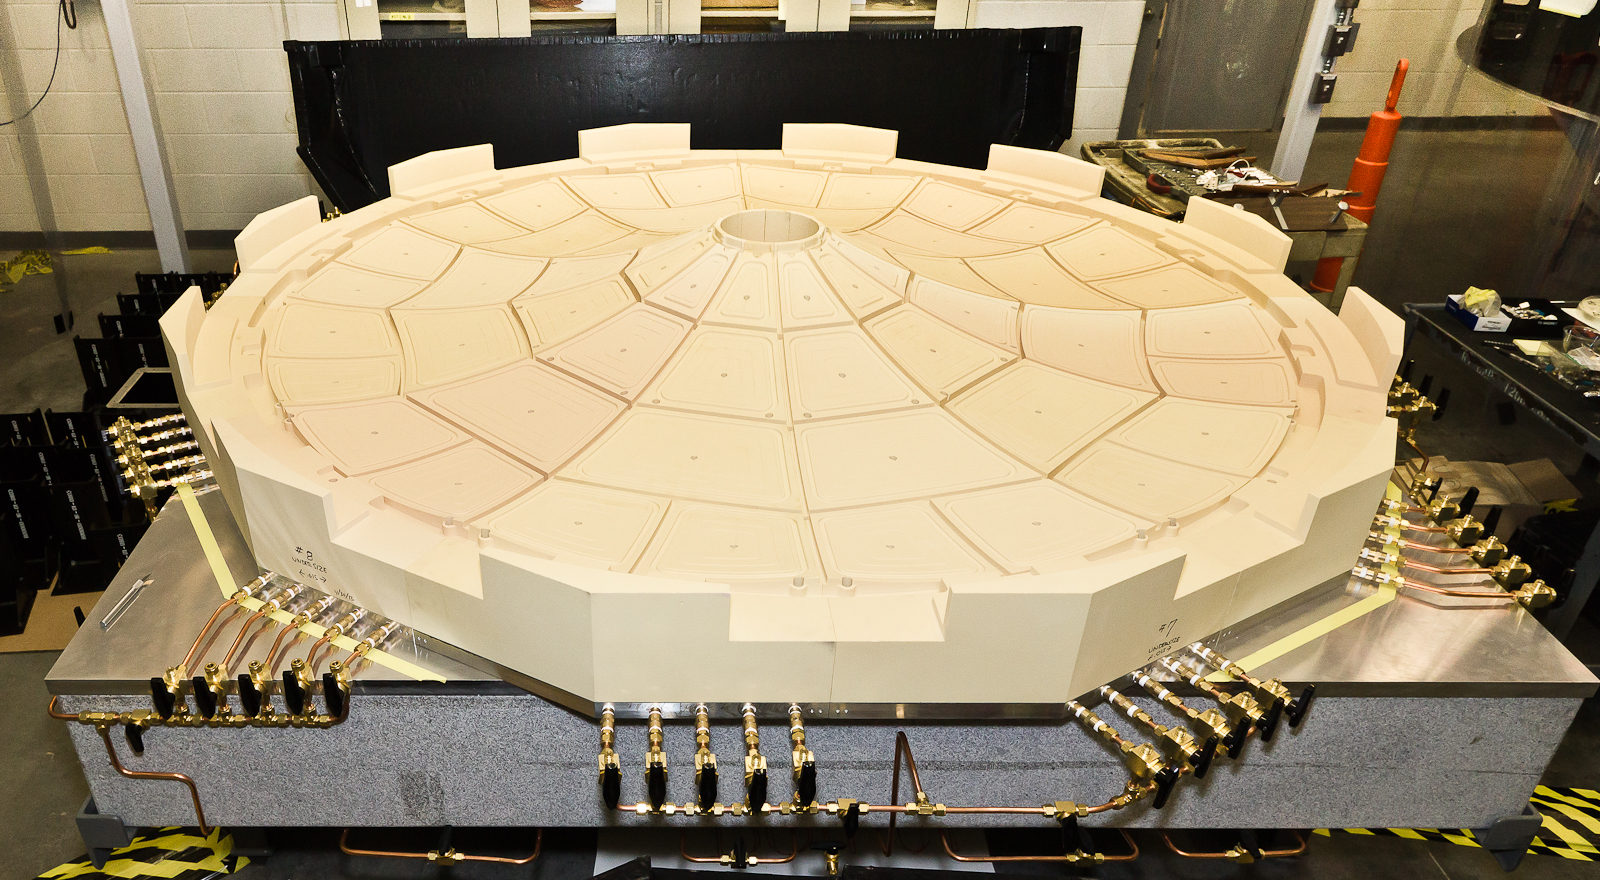
\includegraphics[width=1.0\linewidth]{images/Twelve_Foam_Vacuum_Tables.jpg}
    \caption{All 12 half-sector holding vacuum tables assembled on the 1 inch aluminum plates placed on the granite table}
    \label{fig:Twelve_Foam_Vacuum_Tables}
\end{figure}

\indent It has been decided not to equip the table with any devices to check the geometry of the HTCC mirror during assembly. Since for the assembly we used only 12 half-sectors that have passed the input control and there was not much room available for adjustment of half-sectors on the final assembly table within more than about 0.030" in the radial direction and within gaps between adjacent half-sectors about 0.010", the geometry was already pretty much established and fixed once all 12 half-sectors were hold tight on the table.
\\
\indent The assembly procedure was the same used before for the half-sectors. The only difference was that we had to install in the center of the combined mirror the lightweight central ring (0.055" thick) made of carbon fibers. The ring was glued to all half-sectors. We were controlling and measuring the gaps between all adjacent mirror facets belonging to adjacent half-sectors. Average gap was 0.0096" and is very close to the designed value of 0.008". In fact this is the width of the "dead" zone between half-sectors, i.e. the HTCC mirror covers almost 100\% of azimuthal angular acceptance. It has to be mentioned that the average gaps between adjacent facets in the given half-sector mirror were by 50\% smaller and so providing very efficient coverage of the polar angle acceptance. 

The final assembly of the HTCC combined mirror starts after 100\% completion of the preliminary assembly without using any glue. Then the epoxy glue is applied on the first Half-sector as shown bellow on the Fig.\ref{fig:Ap_Gl_Half_Sect}, the same way as during assembly of the Half-sectors.
 
\begin{figure}[h]
    \centering
    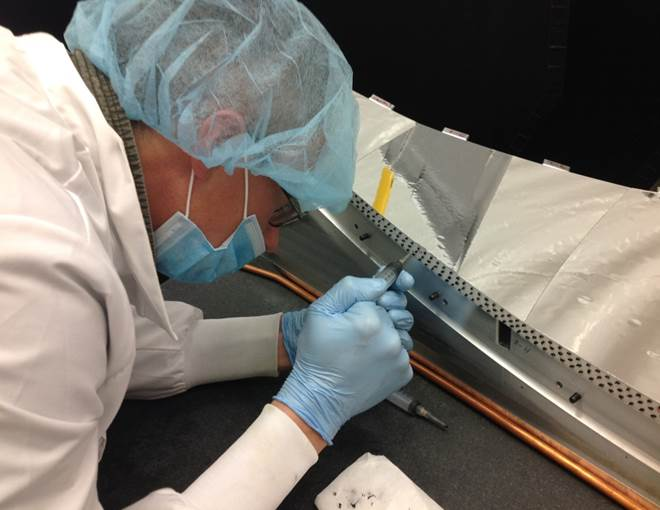
\includegraphics[width=1.0\linewidth]{images/Ap_Gl_Half_Sect.jpg}
    \caption{The dots of epoxy glue are being applied to only one side of the half-sector mirror}
    \label{fig:Ap_Gl_Half_Sect}
\end{figure}
 
 On the Fig.\ref{fig:Partial_Assembl_MIR} is shown the partially assembled combined mirror, and on the nest Fig.\ref{fig:Compl_Assembl_MIR} is shown the final result. 
 
\begin{figure}[h]
    \centering
    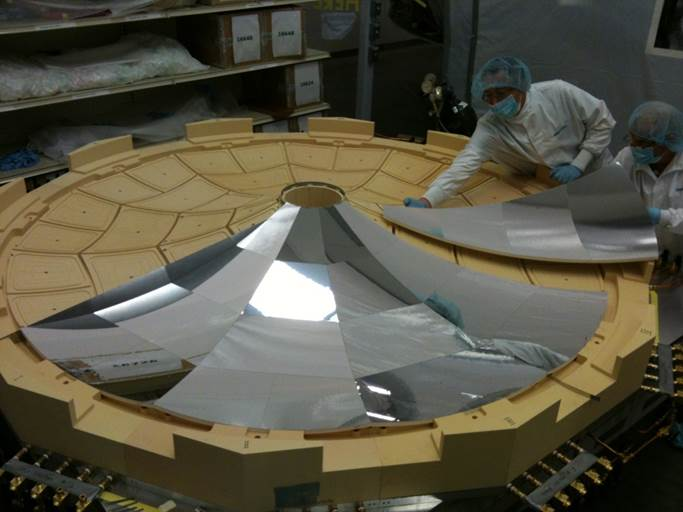
\includegraphics[width=1.0\linewidth]{images/Partial_Assembl_MIR.jpg}
    \caption{ Partially assembled HTCC combined mirror}
    \label{fig:Partial_Assembl_MIR}
\end{figure}

 \begin{figure}[h]
    \centering
    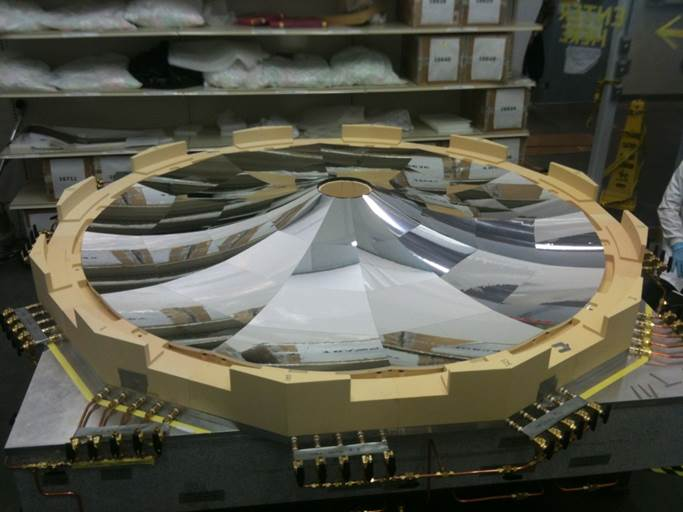
\includegraphics[width=1.0\linewidth]{images/Compl_Assembl_MIR.jpg}
    \caption{Assembled HTCC combined mirror}
    \label{fig:Compl_Assembl_MIR}
\end{figure}

 We used a special procedure to glue the last half-sector because otherwise we would have to be inserting the last half-sector in very narrow place and hence the glue dots will be smeared. Therefore we have assembled first 6 half-sectors on the first 1" mounting plate, and the remaining 6 half-sectors on the other 1" mounting plate. The sides of each group of half-sectors along which they come to contact with each other were free of glue. After that the mounting plates with 6 half-sectors on each were separated from each other by sliding them over the surface the granite table leaving a gap about 1 inch wide, see Fig.\ref{fig:Separated_halves}.
 
  \begin{figure}[h]
    \centering
    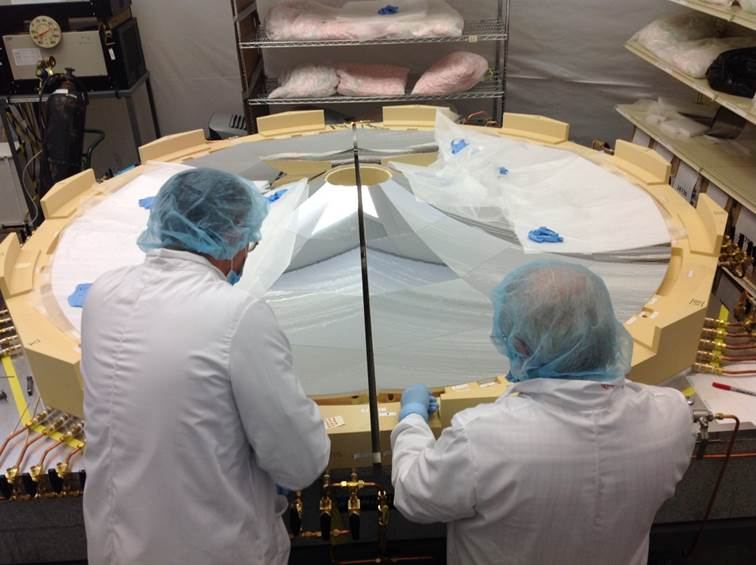
\includegraphics[width=1.0\linewidth]{images/Separated_halves.jpg}
    \caption{Separated halves of the combined mirror before final gluing}
    \label{fig:Separated_halves}
\end{figure}
 
 And then the epoxy glue has been applied to the one of the exposed sides only as it is shown on the Fig.\ref{fig:Final_Gluing}. The last step was to restore the original positions of the plates so that the the both sides come to contact.         
 
   \begin{figure}[h]
    \centering
    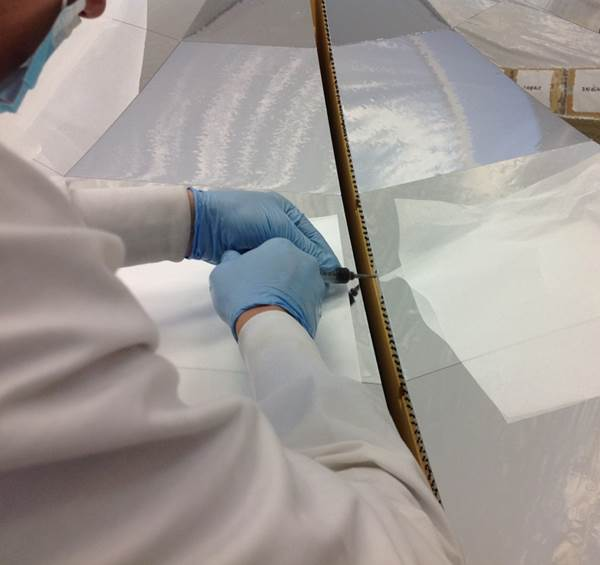
\includegraphics[width=1.0\linewidth]{images/Final_Gluing.jpg}
    \caption{Application of the epoxy glue on the side of the separated halves of the combined mirror to be finally glued}
    \label{fig:Final_Gluing}
\end{figure}
  
  All elements supporting and holding the combined mirror (the ring and bridge pieces) are out of the working acceptance of the HTCC. On the Fig.\ref{fig:Support_Ring} they are shown ready to be attached to the mirror.The rigid lightweight composite supporting ring (strong-back) was attached to the combined mirror via 12 composite lightweight bridge pieces glued to the side around of the mirror. 
  
\begin{figure}[h]
    \centering
    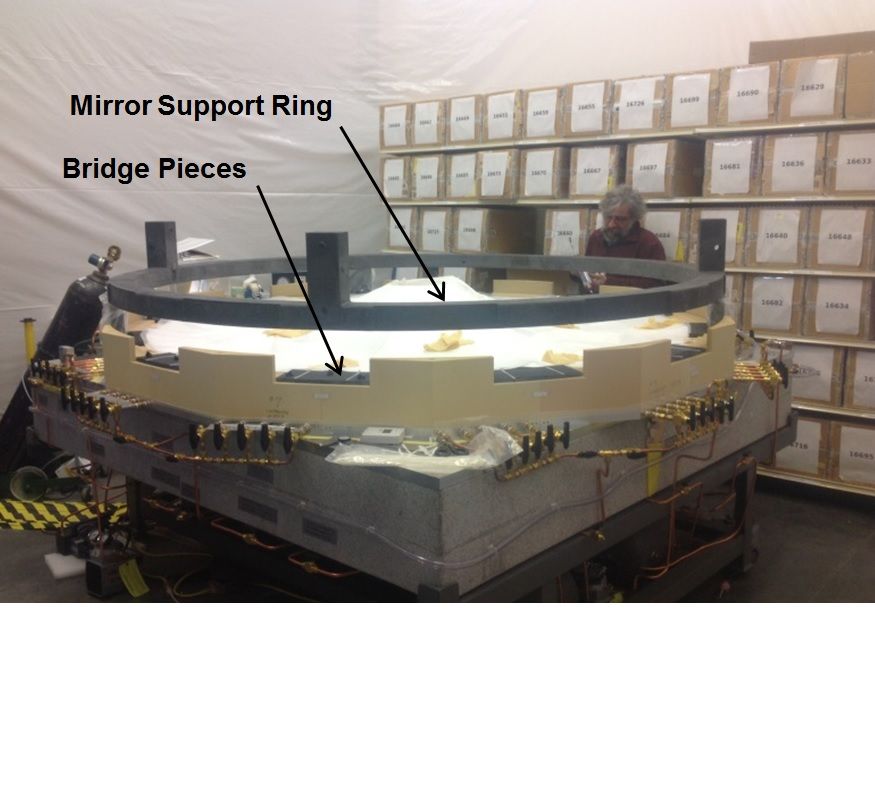
\includegraphics[width=1.0\linewidth,trim={0 5cm 0 0},clip]{images/Support_Ring.jpg}
    \caption{Supporting elements ready to be attached to the combined mirror. The mirror is covered with soft paper towels to protect working surface from debris}
    \label{fig:Support_Ring}
\end{figure}

  Completely assembled HTCC mirror ready for installation is shown on the Fig.\ref{fig:Ring_to_Mirror}. Since the rigidity of the supporting parts is much higher than the rigidity of the combined mirror we used flexible silicon compound for gluing.
  
\begin{figure}[h]
    \centering
    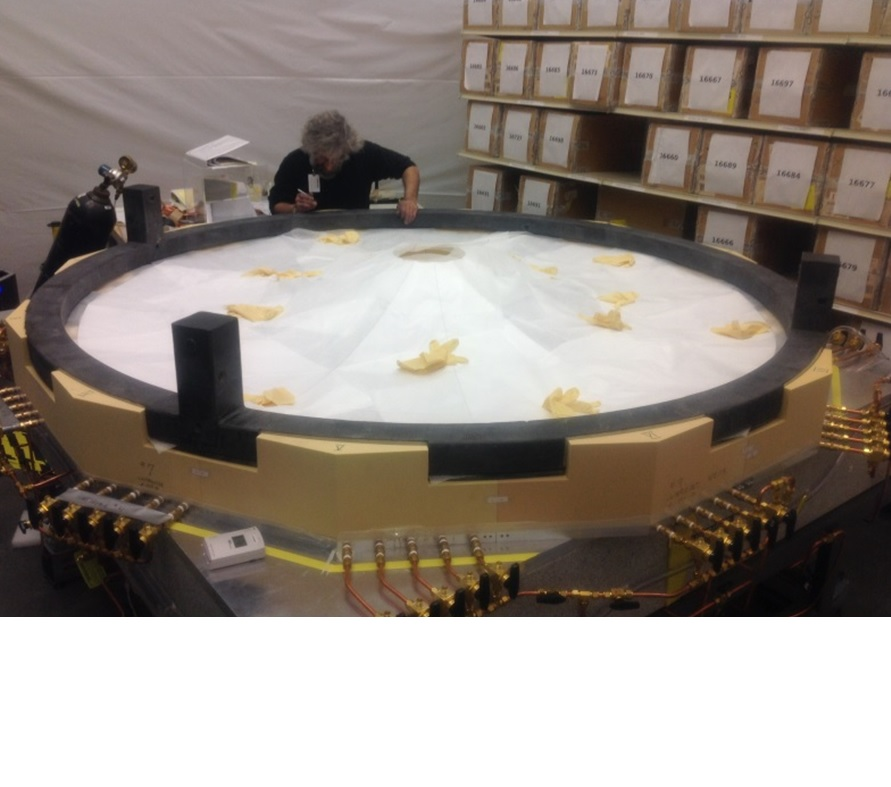
\includegraphics[width=1.0\linewidth,trim={0 5cm 0 0},clip]{images/Ring_to_Mirror.jpg}
    \caption{Completely assembled HTCC mirror ready for installation}
    \label{fig:Ring_to_Mirror}
\end{figure}
 
 
 
 
\subsection {Entry and Exit windows}

\indent There are several aspects that have been taken in consideration that define the design of the entry and exit windows:

\begin{itemize}
    \item Large area to cover
    \item Small thickness
    \item Opaque
    \item High durability
    \item Attachment to the main frame
    \item Structural stability, i.e. resistance to pressure variations
    \end{itemize}

\indent The entry and exit windows are composite films made of three layers of films laminated together: TEDLAR (thickness 38 $\mu$m), MYLAR (thickness 75 $\mu$m), TEDLAR (38 $\mu$m). Composite film was about 61 inches wide and limited by the widths of the other components available. To make the exit window three composite films were glued together side by side. A glue joint between adjacent composite films was made in such a way that the thickness of the joint exceeded the remaining portions by no more than 10\%. The usage of two black TEDLAR films in the composite window guaranteed light insulation even if original film components could possibly have small holes. One layer of Mylar film provided excellent durability and flexibility.
\\
\indent The dimensions of the Entry and Exit windows are of OD $\approx$ 2.5 ft and OD $\approx$ 9.5 ft respectively, so the difference is significant. This required developing a special design of their attachment to the body of the detector. The primary electron beam passes through the HTCC exactly along the axis of the detector. To decrease the background of Moller electrons we have used long shielding made of Tungsten around the beam. It covers a polar angle up to 5$^\circ$ and has a small cylindrical opening in the center that goes all the way through and is big enough for the beam. The working volume of the HTCC must be separated from the volume occupied by Tungsten metal shield. Since the corresponding HTCC part (Moller Cup) concentric to the Tungsten absorber must be lightweight then the joints between this part and the Entry and Exit windows  must also be lightweight. In this case, since the windows have different dimensions, any changes in atmospheric pressure would cause both windows and the Moller Cup attached to them to move upstream or downstream - depending on atmospheric pressure changes. The mirror could be crushed by the Exit window if the pressure goes up, or it could be crushed by conical Moller Cup if the pressure goes down, (see Fig.\ref{fig:side_view}). Thus the Moller cup has to be kept in the same location relative to the mirror regardless of the fluctuations in are atmospheric pressure. Even small changes of $\sim$1 mm of Hg would generate a force of $\sim$200 lbs. acting on the Moller cup along its axis.  

\begin{figure}[h]
    \centering
    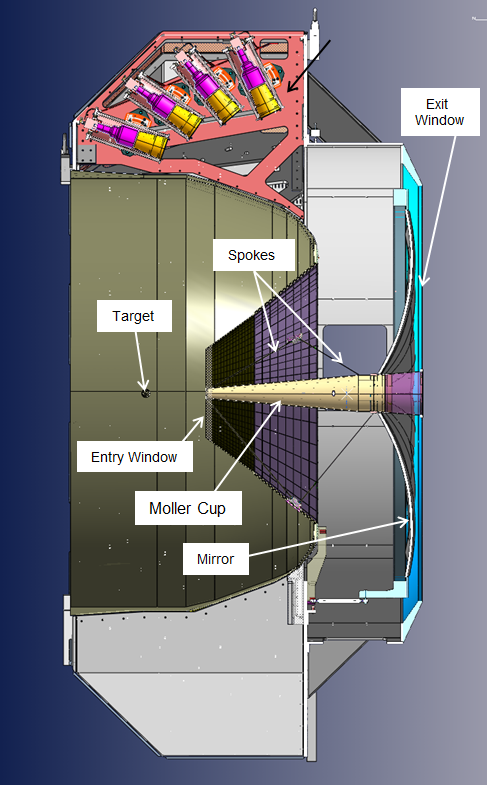
\includegraphics[trim={1.5cm 5cm 0 2cm }, clip, width=\linewidth]{images/Spokes2.png}
    \caption{Side View of the HTCC,  Entry and Exit windows are shown along with other internal components}
    \label{fig:side_view}
\end{figure}

To avoid potential problem with the integrity of the detector the Moller cup was attached to the main frame of the HTCC in 12 points: 6 points on the upstream portion of the main frame, and the remaining 6 points on the downstream portion. All parts providing attachments of the Moller Cup to the front or to the back of the main frame are completely located in the shadow zone of the 6 superconducting coils of the Torus magnet, i.e. they do not create any obstruction to the particles going through the R1, R2 and R3 drift chambers. The Moller cup was attached using 12 thin spokes. Each spoke has OD=1.5mm and was made of carbon fibers to minimize the possible scattering of particles traveling within the shadow of the coils. The spokes very firmly hold the Moller cup in position. All of them are stretched as necessary to provide structural rigidity and to withstand the stresses generated by the attached windows during atmospheric pressure changes. They are stretched as a string in order to eliminate any possible destruction or malfunctioning due to a deformation of the body of the HTCC while transporting, installing or aligning. Each spoke is spring-loaded from both ends. On the Fig.\ref{fig:Front_View} and Fig.\ref{fig:Exit_Win} are presented the upstream and downstream views of the HTCC with installed entry and exit windows.

\begin{figure}[h]
    \centering
    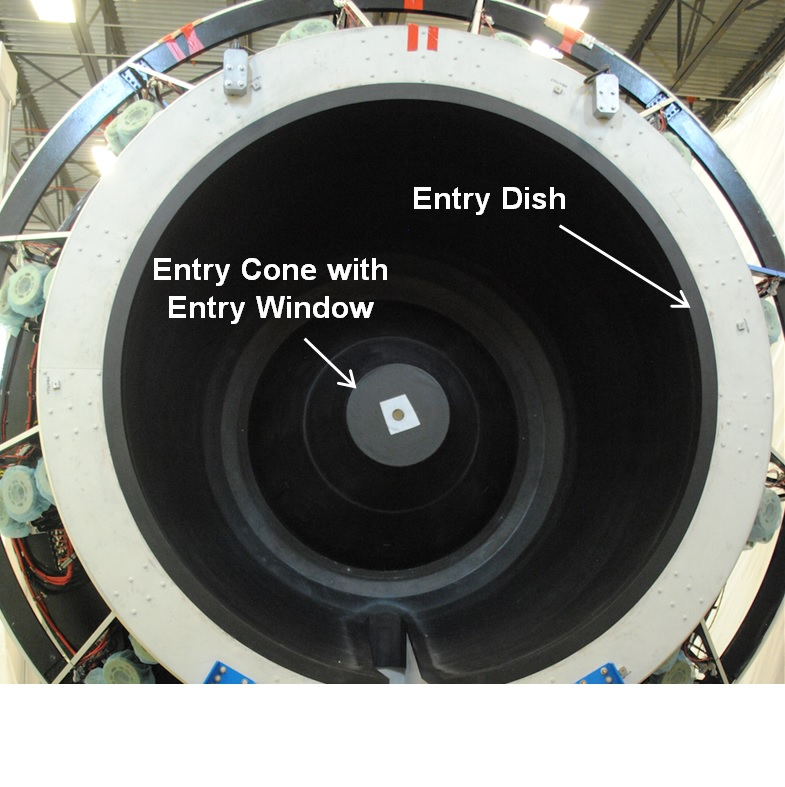
\includegraphics[width=1.0\linewidth,trim={0 2.5cm 0 0},clip]{images/Front_View}
    \caption{Upstream view of the HTCC}
    \label{fig:Front_View}
\end{figure}


\begin{figure}[h]
    \centering
    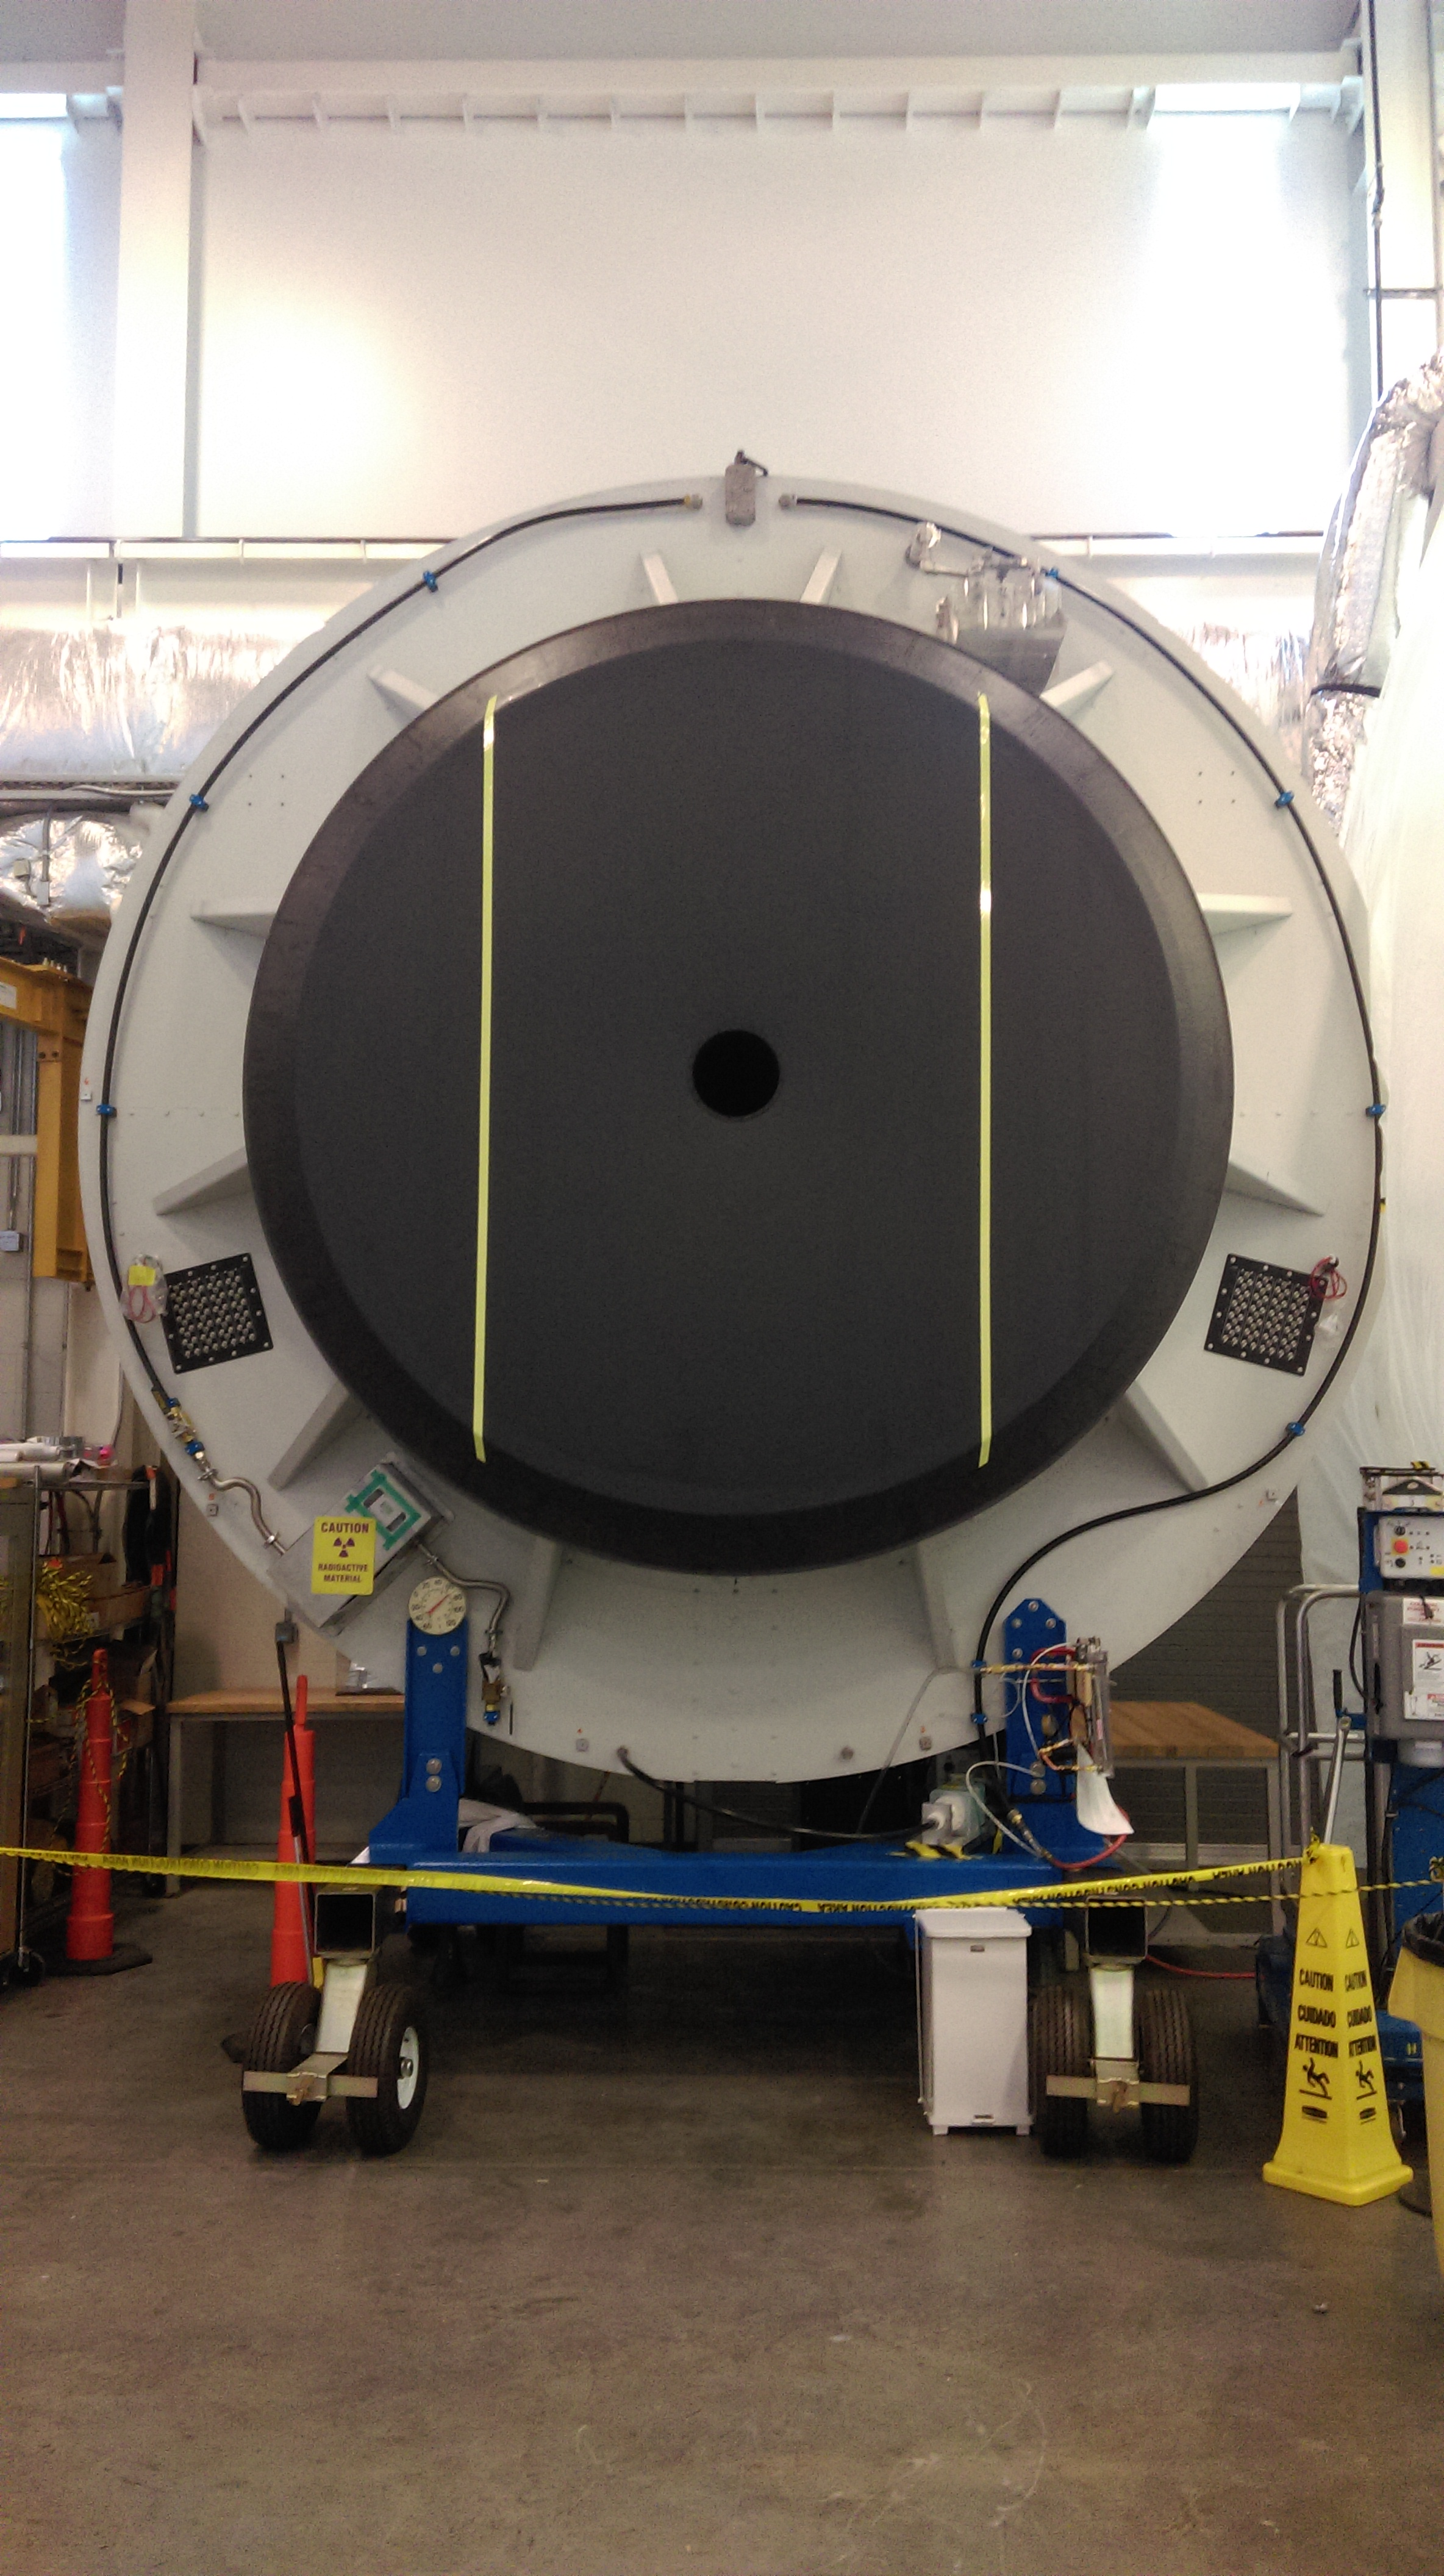
\includegraphics[width=1.0\linewidth,trim={0 25cm 0 500},clip]{images/Exit_Win.jpg}
    \caption{Downstream view of the completely assembled HTCC}
    \label{fig:Exit_Win}
\end{figure}

\subsection{Containment Vessel. Combined Mirror installation}

\indent The Containment Vessel has properties to satisfy a number of requirements, including requirements for the safe transportation of the fully assembled HTCC to the experimental hall without any changes in the alignment of the internal components and the preservation of the mirror integrity. We tested the integrity of the spare mirror by transporting it along the chosen route (see Fig.\ref{fig:transportation_spare_mirror}).

\begin{figure}[h]
    \centering
    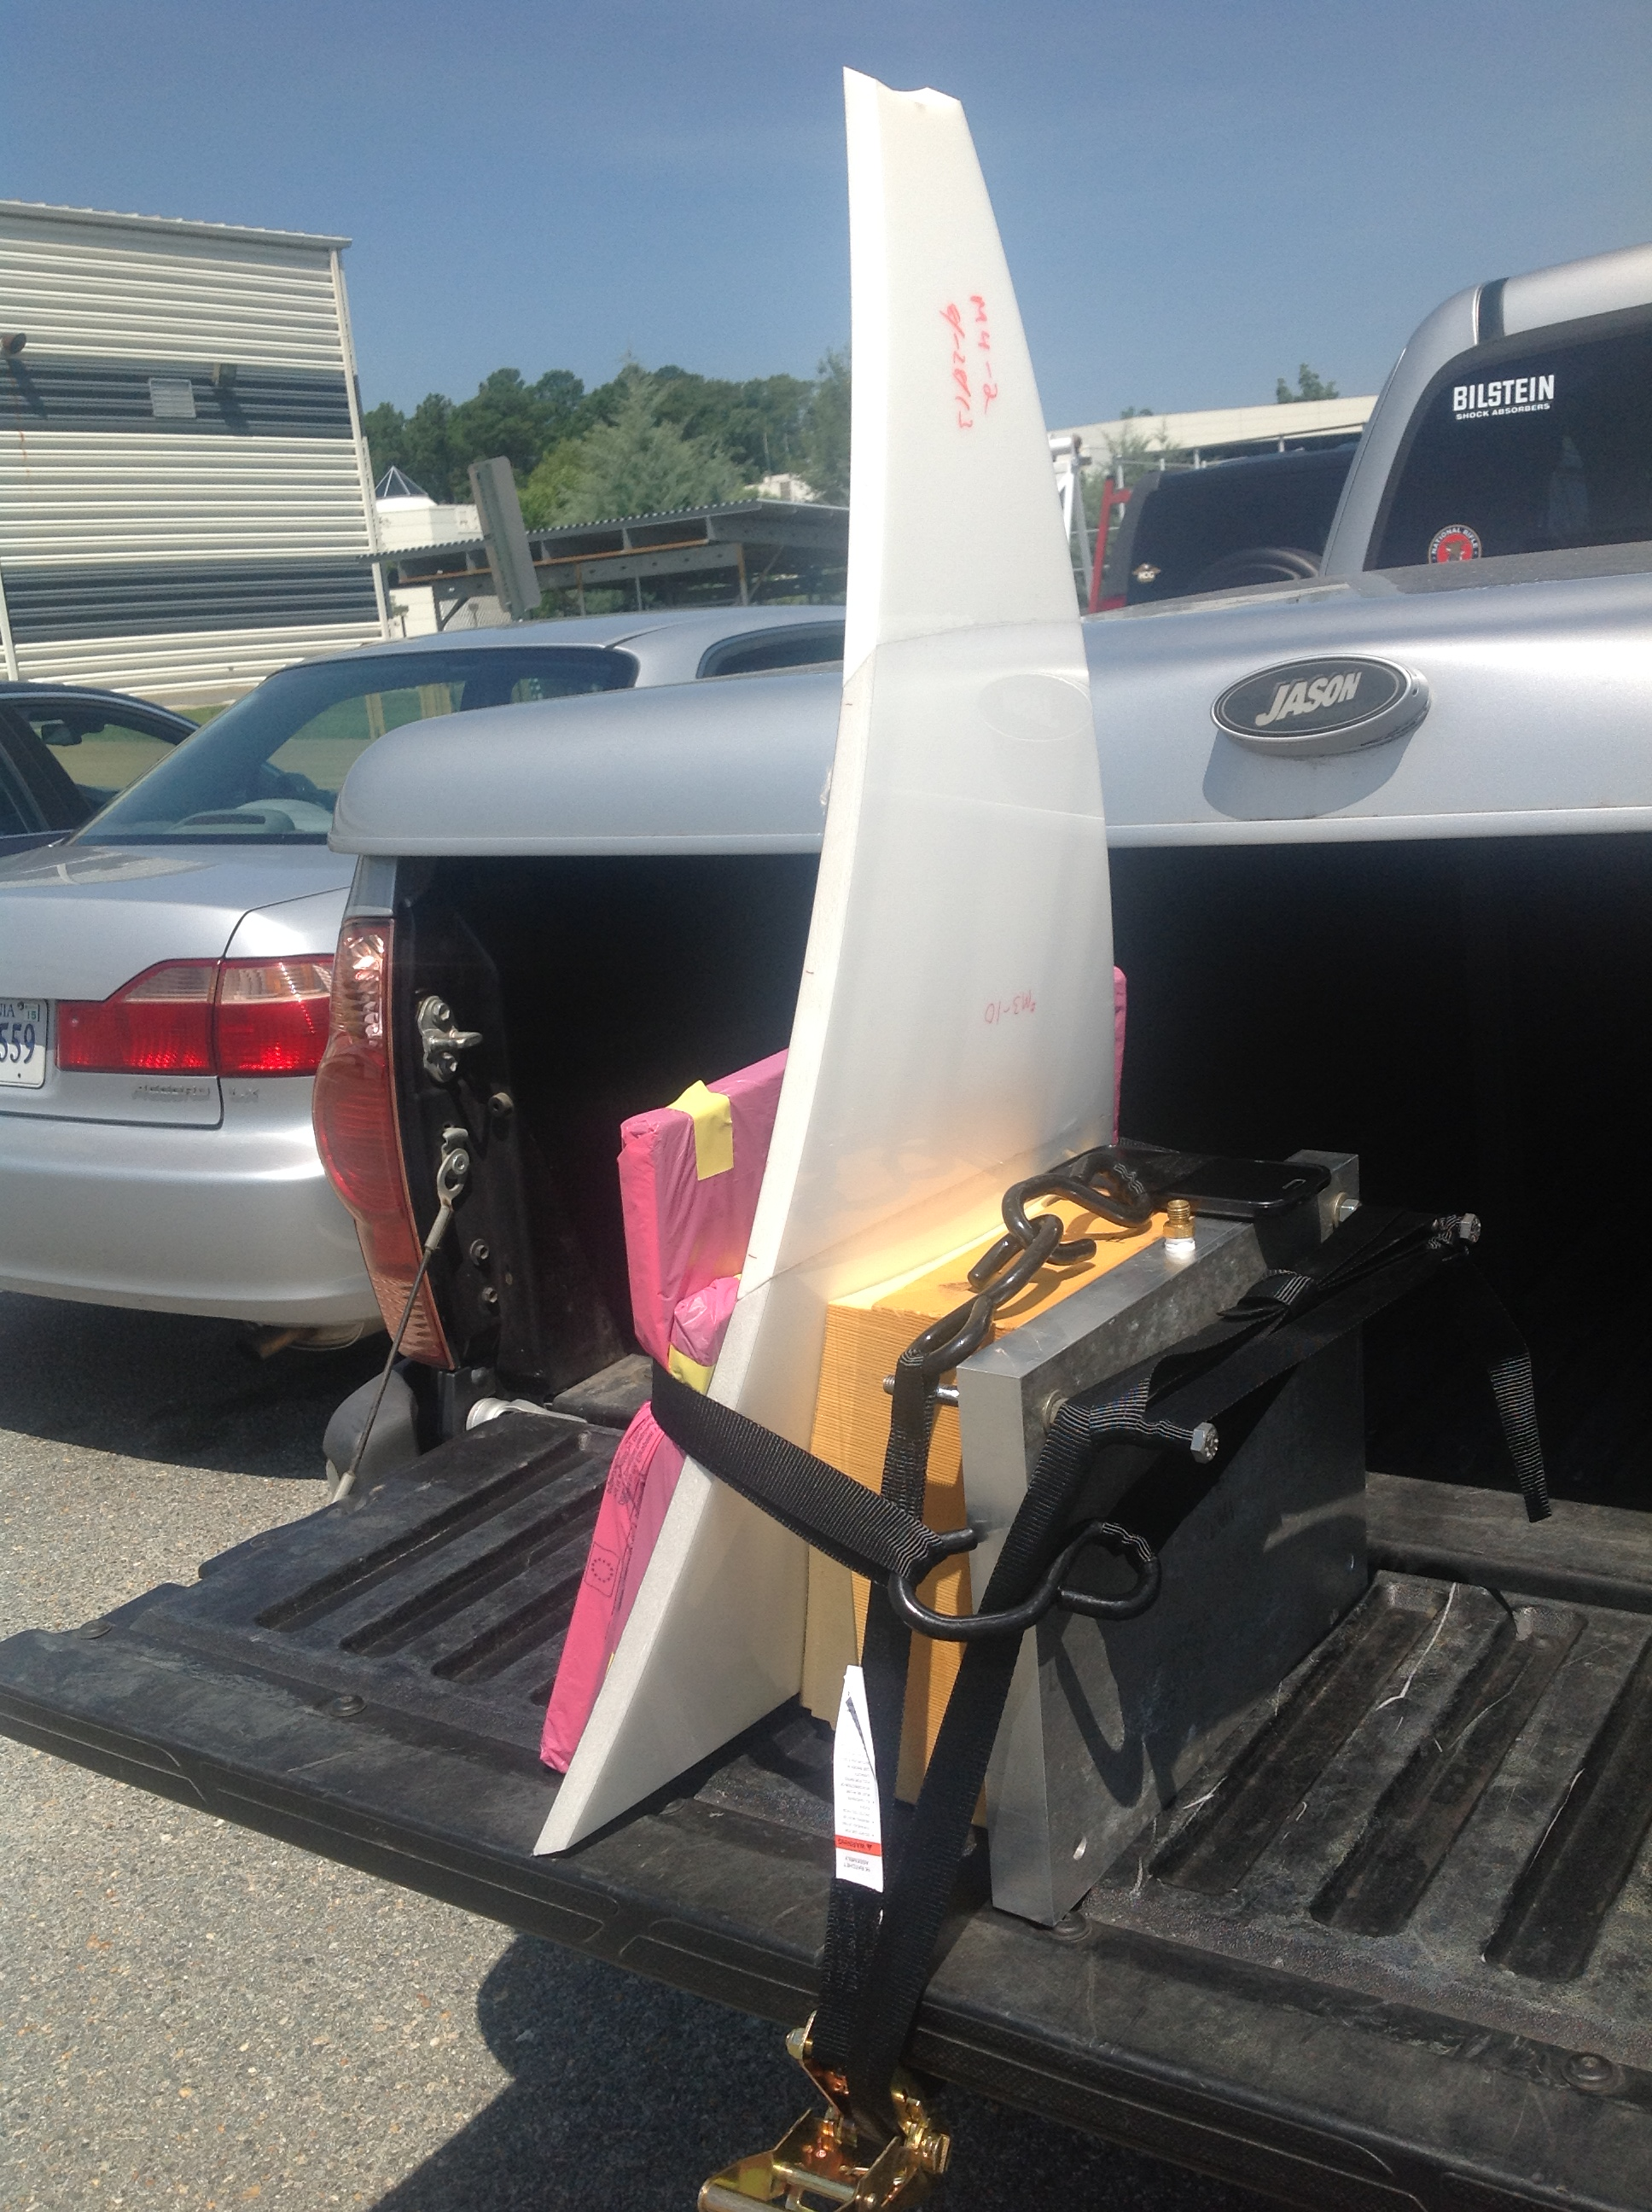
\includegraphics[trim={1.5cm 5cm 0 2cm }, clip, width=\linewidth]{images/Road_Test.JPG}
    \caption{Road Tests of the spare mirror}
    \label{fig:transportation_spare_mirror}
\end{figure}

  Road surface defects caused the mirror to accelerate, and this acceleration was measured at different speeds along the route. The results obtained allowed us to determine the maximum speed with which the detector was supposed to be transported, bearing in mind that it would be exposed to the external environment and, therefore, could be subject to significant temperature changes if the transportation time was not limited in any way. We successfully transported the detector using the results obtained during the test (which included the transportation speed estimates that we obtained). The vessel had to be rigid, have negligible deformation while changing its orientation and, at the same time, allow easy access to any internal component. There is one special requirement for the mirror support structure. The Containment Vessel has only a limited rigidity and is subject to certain deformations. These deformations could directly lead to a dangerous deformation of the HTCC mirror if it was attached to the Containment Vessel in ordinary ways. Even if the mirror remains whole and stays with no cracks the light collection optics would be still changed in a way that would only decrease the signal strength.

\indent In general the vessel works as support structure for all the internal components and must be both light tight and gas tight. Safety considerations require that we have both easy and safe access to the components inside. This is absolutely necessary during maintenance and while running alignment checks. Special attention was paid to the cable and fiber optics routing inside the volume. These items are very difficult to replace. The vessel is equipped with a local gas distribution and a control panel. The control panel is for safe and continuous purging of the volume with different dry gases (as needed) and used to keep the water vapors concentration level under tight control during both  operations and maintenance.

\indent The HTCC combined mirror is supported and hold in the containment vessel by 6 orthogonal links. These links connect the supporting ring (with the attached to it combined mirror) to the containment vessel.
\indent It was critical that any deformation that might be taking place in the containment vessel not be transmitted to the combined mirror. Each link has a ball end swivel on each end. By using the minimum number of links (6) which constrain all motions, the mirror could be aligned, but no forces above those due to gravity of the mass of the mirror and its strong-back are ever placed on the mirror. Set of links are attached to the containment vessel in 3 points that are 120$^\circ$ spaced around the perimeter of the ring. With regard to the installation of the mirror the tests using very lightweight flat mirror of relatively large diameter of about 5 ft. have been conducted. The tests have shown that the light collection pattern stays unchanged within sufficiently wide range of deformations of the frame that was supporting the flat test mirror. Therefore possible deformation of the containment vessel during installation and alignment do not affect the original shape of the HTCC mirror. 

On the Fig.\ref{fig:HTCC_MIRR_INST} is shown the HTCC mirror installed in the containment vessel the way described above.

\begin{figure}[h]
    \centering
    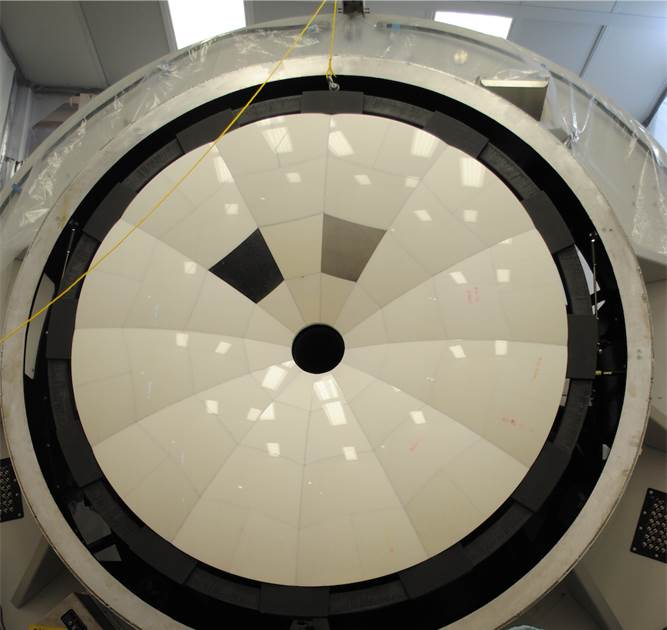
\includegraphics[width=1.0\linewidth,trim={0 0cm 0 0},clip]{images/HTCC_MIRR_INST.jpg}
    \caption{Combined Ellipsoidal Mirror installed in the Containment Vessel. Set of links holding the Mirror in the position allow fine adjustment with accuracy of ~ 0.01 inch or better}
    \label{fig:HTCC_MIRR_INST}
\end{figure}

\indent The HTCC is susceptible to noticeable deformations due to the detector's large overall dimensions.The light and gas protections that are provided thus had to be reliable and require little maintenance. All the inside surfaces have been painted a flat black to reduce light reflectance. All the borders between adjacent parts that form the outside shell of the detector have been sealed with a flexible black silicone gel on both the inside and outside of the vessel. Sealing all the inside seams is necessary because the detector would thus always stay under a positive differential pressure that is continuously changing due to variations in the atmospheric pressure. As a result of even small changes in the differential pressure, the vessel would be deformed due to its large volume, i.e.the pressure is applied to a large surface. 

\subsection{Alignment of the Light Collection Components}
The HTCC contains light collection and light detection components: the mirror, Winston Light Concentrators, photomultiplier tubes. Even if the mirror is constructed and installed properly as designed the final checks of the components alignment are needed. We have conducted comprehensive checks of the light collection optics on the fully assembled detector. This work has been done before the detector was moved to the experimental hall. For the alignment checks we used again the low power laser gimbal mounted in the target position. To operate the laser we used set of standard high precision devices to control position and orientation of the laser. The opaque entry window was replaced with thin transparent film in order the volume of the detector stay still isolated as much as possible when needed. We were opening one hatch at the time for short period of time to install templates on the face of accessible Winston cones and perform adjustments of the PMT housing units each containing 5-inch PMT, Winston cone, 3-layer magnetic shield and compensation coil. Alignment of all 48 PMT housing units were checked and adjusted as needed. Each mirror facet has been illuminated with laser in 5 points: the center of the facet and four corners. Reflected light  pattern was photographed. For some of the most important channels, i.e. of those which monitor mirror facets covering small polar angles up to $20^\circ$, we have checked the light collection geometry at normal relative humidity in the HTCC volume and at 0\% relative humidity. We allowed enough time for components to rich the required equilibrium.

On the Fig.\ref{fig:GEO_TEST_3_Normal} is shown pattern of the light reflection when mirror facet \#3 was illuminated in the center. The circles of diameter 1", 3" and 5" concentric to the PMT are shown. The result was obtained at normal relative humidity. Results obtained at RH=0\% for the same channel is shown in the Fig.\ref{fig:GEO_TEST_3_Zero}. As one can see there is small but acceptable difference. Similar geometry test results have been obtained for the channel \#4 covering polar angles in range of $5^\circ$ to $12.5^\circ$. They are presented in the Fig.\ref{fig:GEO_TEST_4_Normal} and  Fig.\ref{fig:GEO_TEST_4_Zero} obtained correspondingly at normal and low relative humidity.

\indent Considering the light collection patterns obtained when mirror facets were illuminated in the corners we made all necessary adjustments in the alignment of the PMT mounting units. No adjustments were needed for the HTCC mirror. On the Fig.\ref{fig:Ch_5_1_3_Before} are shown test results for the mirror facet \#3 from Sector 5, Half-Sector 1 obtained before adjustments in alignment was done. Data were fitted and presented on the Fig.\ref{fig:Ch_5_1_3_Before} as well. On the Fig.\ref{fig:Ch_5_1_3_After} one can see changes in the light collection pattern after adjustment in alignment. The image has been shifted toward the center. On the next Fig.\ref{fig:GEO_TEST_5_1_3_Center} this is demonstrated by illuminating the mirror in the center. Five circles concentric to the PMT shown in the picture are 1" to 5" of diameter. 


\begin{figure}[h]
    \centering
    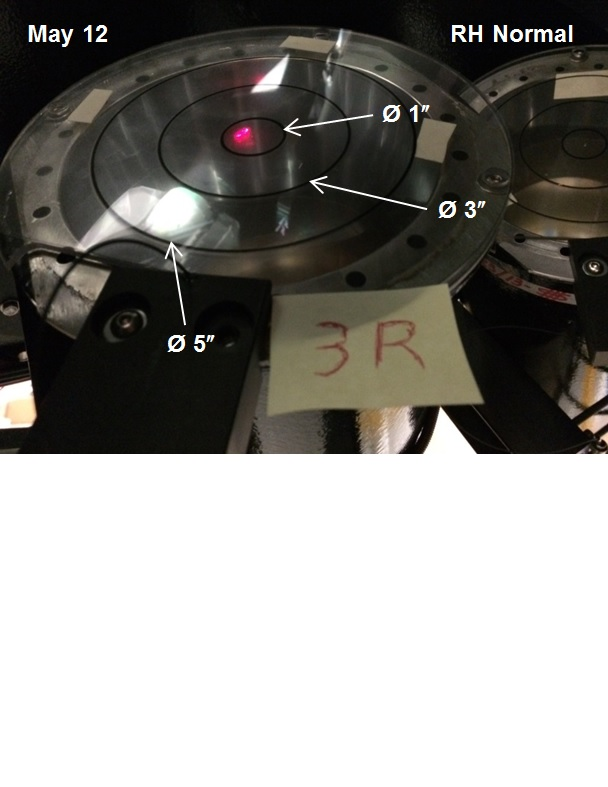
\includegraphics[width=1.0\linewidth,trim={0 8.5cm 0 0},clip]{images/GEO_TEST_3_Normal.jpg}
    \caption{Geometry test result for the channel covering polar angles in range of $12.5^\circ$ to $20^\circ$. Corresponding mirror facet was illuminated in the center}
    \label{fig:GEO_TEST_3_Normal}
\end{figure}

\begin{figure}[h]
    \centering
    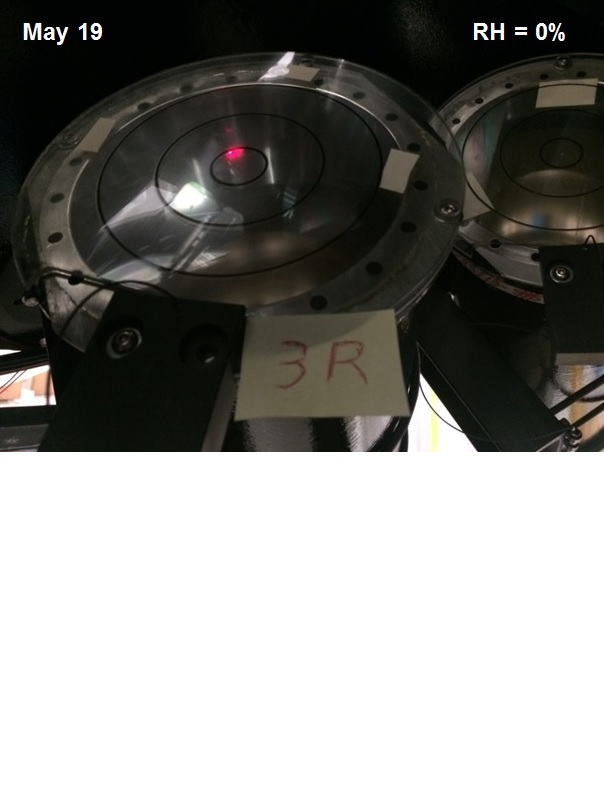
\includegraphics[width=1.0\linewidth,trim={0 8.5cm 0 0},clip]{images/GEO_TEST_3_Zero.jpg}
    \caption{Geometry test result for the channel covering polar angles in range of $12.5^\circ$ to $20^\circ$ obtained at RH=0\%. Corresponding mirror facet was illuminated in the center}
    \label{fig:GEO_TEST_3_Zero}
\end{figure}
        
\begin{figure}[h]
    \centering
    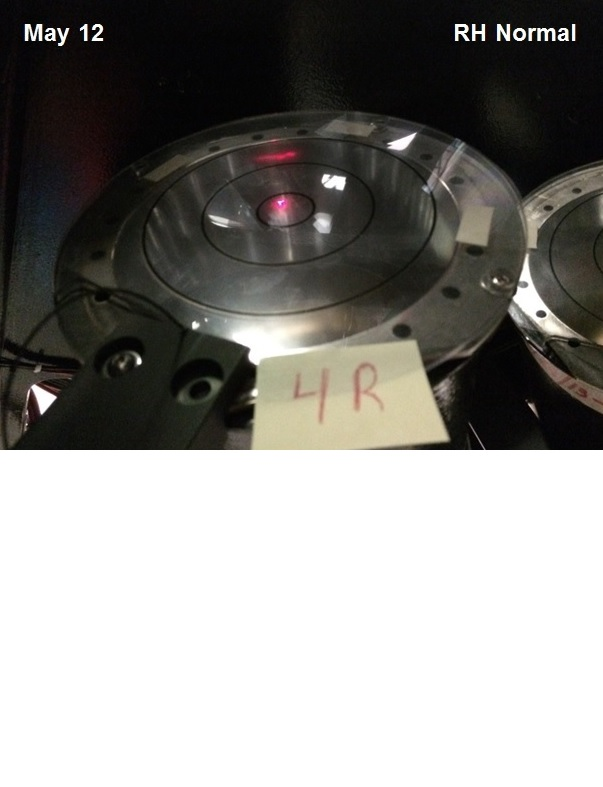
\includegraphics[width=1.0\linewidth,trim={0 8.5cm 0 0},clip]{images/GEO_TEST_4_Normal.jpg}
    \caption{Geometry test result for the channel covering polar angles in range of $5^\circ$ to $12.5^\circ$. Corresponding mirror facet was illuminated in the center}
    \label{fig:GEO_TEST_4_Normal}
\end{figure}

\begin{figure}[h]
    \centering
    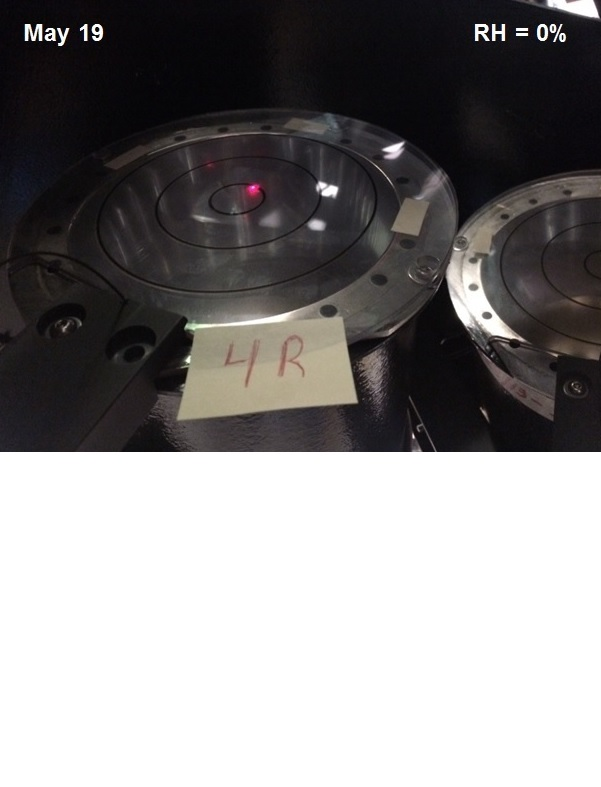
\includegraphics[width=1.0\linewidth,trim={0 8.5cm 0 0},clip]{images/GEO_TEST_4_Zero.jpg}
    \caption{Geometry test result for the channel covering polar angles in range of $5^\circ$ to $12.5^\circ$ obtained at RH=0\%. Corresponding mirror facet was illuminated in the center}
    \label{fig:GEO_TEST_4_Zero}
\end{figure}

\begin{figure}[h]
    \centering
    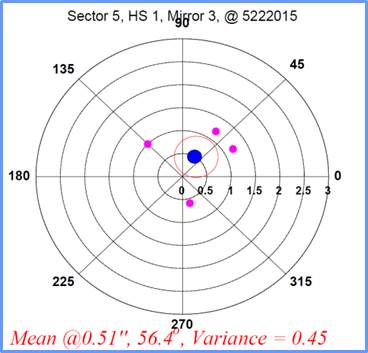
\includegraphics[width=1.0\linewidth,trim={0 0cm 0 0},clip]{images/Ch_5_1_3_Before.jpg}
    \caption{Geometry test result for the Sector 5, HS 1, Mirror \#3 covering polar angles in range of $12.5^\circ$ to $20^\circ$ obtained before adjustment when mirror \#3 was illuminated in the corners}
    \label{fig:Ch_5_1_3_Before}
\end{figure}

\begin{figure}[h]
    \centering
    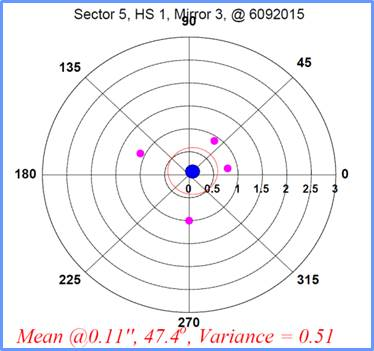
\includegraphics[width=1.0\linewidth,trim={0 0cm 0 0},clip]{images/Ch_5_1_3_After.jpg}
    \caption{Geometry test result for the Sector 5, HS 1, Mirror \#3 covering polar angles in range of $12.5^\circ$ to $20^\circ$ obtained after adjustment when mirror \#3 was illuminated in the corners}
    \label{fig:Ch_5_1_3_After}
\end{figure}

\begin{figure}[h]
    \centering
    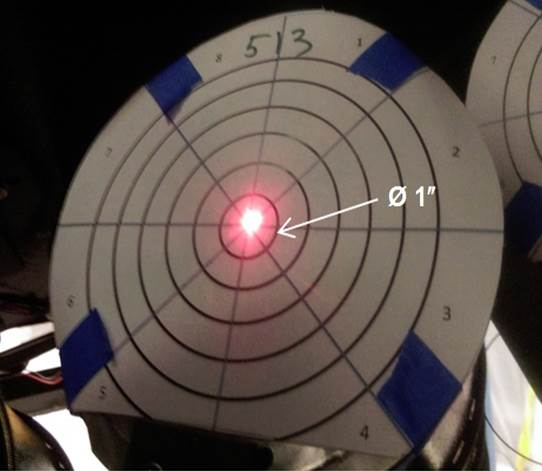
\includegraphics[width=1.0\linewidth,trim={0 0cm 0 0},clip]{images/GEO_TEST_5_1_3_Center.jpg}
    \caption{Geometry test result for the Sector 5, HS 1, Mirror \#3 covering polar angles in range of $12.5^\circ$ to $20^\circ$ obtained after adjustment when mirror \#3 was illuminated in the corners}
    \label{fig:GEO_TEST_5_1_3_Center}
\end{figure}

In the Fig.\ref{fig:subfig} are brought data on the final light collection patterns obtained for all mirrors for HS1 and HS2 from Sector 5. One can clearly see that the light collection is more focused for the small mirrors than for large ones. This effect is caused by difference between combined mirror itself and supporting ring attached to it regarding their rigidity and sensitivity to the changes in relative humidity of the environment they are surrounded. As we have observed the fully assembled combined mirror wood stay similar to itself with relatively small changes in its overall dimensions  if relative humidity is changing from normal to low. The support ring is insensitive to such humidity changes. This two components are glued together with glue which is relatively elastic as compared with epoxy. But still changes in diameter of the mirror due to humidity generates a certain force stretching the relatively elastic glue joint between ring and the mirror. In other words the mirror is being radially stretched. Since the mirror has a shape of funnel, see Fig.\ref{fig:Colored_Mirror}, than the nose of the funnel gets stretched less than outer portion of the mirror. The outer portion of the mirror is mostly consists of mirror facets \#1 and \#2, the largest mirror facets. Even the widths of facet \#1 and \#2 measured in in radial direction are close to each other effect of humidity change for the outermost facet \#1 is larger than for facet \#2 all due to the funnel shape of the combined mirror.

\begin{figure*}
\begin{subfigure}[b]{0.49\textwidth}
    \includegraphics[width=1.0\textwidth]{images/GEO_TEST_Sect5_M_1_M_2.jpg}
    \caption{Mirrors \#1 and \#2 are covering polar angles in range of $20^\circ$ to $35^\circ$  within azimuthal interval of $60^\circ$} \label{fig:subfig1_a}
\end{subfigure}
\hspace*{\fill} % separation between the subfigures
\begin{subfigure}[b]{0.5\textwidth}
    \includegraphics[width=1.0\linewidth]{images/GEO_TEST_Sect5_M_3_M_4.jpg}
    \caption{Mirrors \#3 and \#4 are covering polar angles in range of $5^\circ$ to $20^\circ$  within azimuthal interval of $60^\circ$} \label{fig:subfig1_b}
\end{subfigure}
\caption{Light collection test result for both half-sectors of the Sector 5. Data are obtained after adjustment. The mirrors were illuminated in the center and corners} 
\label{fig:subfig}
\end{figure*}

\begin{figure}[h]
    \centering
    \includegraphics[width=1.0\linewidth,trim={0 0cm 0 0},clip]{images/Colored_Mirror.jpg}
    \caption{HTCC combined multifocal ellipsoidal  mirror}
    \label{fig:Colored_Mirror}
\end{figure}


\subsection{Gas Composition Control}
\indent The fully assembled detector has been tested for gas and light leaks. Gas tightness was checked by filling the volume with mixture of dry air and of small amount of non-flammable gas at positive differential pressure. Freon gas leak sniffers were used. As expected, most of the leaks were found and around the entry and exit windows. This is because both windows have been sealed only from the outside as they were the last two components that had been attached to the containment Vessel. Light tightness was checked by monitoring the counting rates of the photomultiplier tubes while illuminating the sealed seams of the vessel with an external light source. The rates were close to the dark counting rates whether the lights in the hall were turned on or off. The gas tightness was controlled by fixing leaks found and then by measuring humidity inside the detector while it was continuously purged with a dry nitrogen. At rates of 10 - 15 L/min the stable level not higher than $\sim$ 100 ppm of humidity had been established in span of 2-3 days of continuous purging. These results can be used as a good indication of a low level of water vapor content and of oxygen as well [A]. This is because of design and materials used in composite windows manufacturing. The windows are made of two layers of TEDLAR films with one layer of MYLAR film between them which are then laminated together. TEDLAR films are absolutely opaque and thus the use of two layers guarantees that there are no holes. The diffusion of water vapors and oxygen through the windows is defined by TEDLAR, which has the lowest diffusion coefficients. For TEDLAR the diffusion of oxygen is lower than the diffusion of water vapors. The presence of water vapors and of oxygen in the working volume is unavoidable but should be kept at the lowest possible level because the water vapors and CO${_2}$ gas produce carbonic acid that may be harmful to the mirror working surface. The stable level of $\sim$100 ppm or less of water vapor corresponds to less than 1\% of the relative humidity, but the relative humidity also depends on the temperature. This makes it harder to interpret any changes in the actual readings.
\\
\indent As far as oxygen content is concerned its level also needs to be kept at the lowest possible level. During operations with beam a certain amount of ozone can be generated due to radiation.This two gases oxygen and ozone absorb the ultraviolet component of Cerenkov light in the HTCC generated by scattered electrons. Consequently the signal strength becomes lower which directly leads to a poor, or to at least worse than expected, rejection of background charged pions.

Almost one year has passed since CLAS12 operations with beam started, and no degradation of signal strength has been observed. At least this means that all controlled parameters are stable. But still actual composition and possible changes of the radiator gas is unknown. We plan installation of the residual gas analyzer to  continuously monitor the concentration of oxygen, ozone and helium gases. Helium is especially harmful for the PMTs with quartz windows. Quartz entry windows are freely penetrated by helium gas, and the introduction of helium would ruin the vacuum in the PMT. The ozone and helium are generated during running experiments. The ozone is due to radiation, and the presence of helium is due to the operations of the superconducting Torus magnet and Central Solenoid magnet in the hall. Since more than 50\% of the containment vessel surface are covered with plastics the only tool to better control gas composition would be usage of the reasonably high rate of purging.
\\
\indent Another reason to keep tight control on humidity is related to the sensitivity (to some extent) of the mirror shape to humidity. The mirror must be used at the lowest humidity level, but the entire manufacturing process of mirror facets had to be done at normal room conditions. Once the mirror had been installed, the HTCC volume was sealed and purged with dry gas (N${_2}$, CO${_2}$ or dry air depending on the hall's status). The mirror is kept at the lowest humidity. Altering the humidity from almost zero to normal may lead to fatigue and cause structural deformation. During maintenance the volume is partially exposed to the outside environment, which increases humidity. In any case, all the maintenance activities we stop once inside the volume relative humidity reaches 2-3\%. This is controlled at the exhaust of the detector. Maintenance is resumed only after the operational humidity level is restored. The detector is equipped with a local gas control panel, which is attached to the side of the HTCC. The parameters that can be read directly are limited to the pressure at the input of the volume and the differential pressure. We also use a device that allows us to visually observe if humid gas is or was used during purging. The HTCC is continuously monitored online by a system control by checking the following parameters:

\begin{itemize}
    \item Type of gas
    \item Gas flow rate
    \item Differential pressure
    \item Humidity
    \item Amount of gas already consumed
\end{itemize}

\indent  The online control system allows for safely operating the detector within predefined intervals of parameter variations. This system generates warnings and alarms that require quick remote or in situ response. In the case of a power outage in the hall, the Mass Flow Controller turns off and purging is stopped. It takes several hours for the humidity to rise up to 2-3\% due to direct leaks and diffusion of the ambient humid air inside the working volume. This is enough time to switch the gas flow from not energized Mass Flow Controller to a manual bypass rota-meter, which is normally closed. The local gas panel includes three specialized filters that prevent the dust, water vapors and oil vapors from entering the volume.

\indent There was a need to have easy access to any of 48 PMTs to adjust their alignment (See Subsection describing alignment) and for maintenance. The Containment Vessel has 24 service hatches wide enough for two people to perform any work with any channel. Each channel consists of a PMT wit high voltage divider, magnetic shield with compensation coil and Winston Cone. They are installed in the PMT mounting fixture together as one unit, see Fig.\ref{fig:PMT_Mount}.

\begin{figure}[h]
    \centering
    \includegraphics[width=1.0\linewidth,trim={0 12cm 0 0},clip]{images/PMT_Mount.jpg}
    \caption{PMT mounting unit with components}
    \label{fig:PMT_Mount}
\end{figure}

Checks of cabling and installed fiber optics are used for calibration of the PMTs. These can be done with external light source (see Section ... for details) and also be done using aforementioned hatches. All necessary service work can be performed on the detector while it is in nominal working location. Any access to the internal components of the detector require replacement of the working gas with dry oxygen. For safety the corresponding procedure of purging the HTCC volume has been established to only allow access in case of when the concentration of oxygen in the volume exceeds 19.5\%.
